\documentclass{article}

\usepackage{fullpage}
\usepackage{doublespace}
\usepackage{epsfig}

\title{A Stream Compiler for Communciation-Exposed Architectures}

\author{Michael Gordon, William Thies, Michal Karczmarek, Jeremy Wong, \\
  Henry Hoffmann, David Maze and Saman Amarasinghe\\ \\
  MIT Laboratory for Computer Science\\
  Cambridge, MA  02139\\ \\
  \sffamily{\{mgordon, thies, karczma, jnwong, hank, dmaze, saman\}@lcs.mit.edu}}

% don't include the date
\date{}

% this is the line spacing
\setstretch{1.75}

% \sloppy lets Latex be a little less anal about interword spacing.  It is
% one way to eliminate those annoying Overfull hbox warnings.
% Another way is to surround each offending paragraph with
% \begin{sloppypar} ... \end{sloppypar}

%\sloppy

% See page 90 of the Latex book for info about vertical spacing probs.

\begin{document}

  \newcommand{\todo}[1]{\framebox{#1}}

  %\toappear{\centerline{\Large\bf MIT LCS Technical Memo,}
  %          \centerline{\Large\bf MIT-LCS-TM-6XX,}
  %          \centerline{\Large\bf November, 2001.}}
  
  \begin{singlespace}
    \maketitle
    \begin{abstract}
      Due to the high data rates involved in audio, video, and signal
processing applications, it is imperative to compress the data to
decrease the amount of storage used.  Unfortunately, this implies that
any program operating on the data needs to be wrapped by a
decompression and re-compression stage.  Re-compression can incur
significant computational overhead, while decompression swamps the
application with the original volume of data.

In this paper, we present a program transformation that greatly
accelerates the processing of compressible data.  Given a program that
operates on uncompressed data, we output an equivalent program that
operates directly on the compressed format.  Our transformation
applies to stream programs, a restricted but useful class of
applications with regular communication and computation patterns.  Our
formulation is based on LZ77, a lossless compression algorithm
utilized by ZIP, and immediately applies to simpler formats such as
Apple Animation, Microsoft RLE, and Targa.

We implemented a simple subset of our techniques in the StreamIt
compiler, which emits executable plugins for two popular video editing
tools: MEncoder and Blender.  For common operations such as color
adjustment and video compositing, computing directly on compressed
data offers a speedup roughly proportional to the overall compression
ratio.  For our benchmark suite of 12 videos in Apple Animation
format, speedups range from 1.1x to 471x, with a median of 15x.

    \end{abstract}
  \end{singlespace}
  
  \section{Introduction}


Stream computing represents an increasingly important class of
applications. In streaming codes, there is an abundance of parallelism that
is easier to extract compared to traditional desktop workloads (e.g.,
pointer-based computing). As a result, the extraction of parallelism
in streaming codes does not require heroic efforts, and thus,
processors can deliver higher performance with significantly lower
power costs. This is especially important since
leading microprocessor companies have realized that modern general
purpose architectures are near their  performance limits for  the
amount of power they consume. Thus, the future will place a greater
emphasis on exploiting the properties of streaming workloads in
conventional von~Neumann architectures.

Streaming is a model of computation that uses sequences of data
and computation kernels to expose concurrency and locality for
efficiency~\cite{wss}. In general purpose processors, improving locality 
translates to an effective management of the memory hierarchy at all
levels, including the register file. In this paper, we present a
methodology for compiling streaming codes to general purpose,
cache-based architectures. We first introduce a simple model for
reasoning effectively about the caching behavior of streaming
workloads. This model serves as a foundation for several {\it cache-aware
optimizations} that are geared toward the concomitant increase of instruction
and data {\it temporal locality}. These
optimization lead to significantly better utilization of the memory
system, and as such, they deliver performance gains ranging from 11
to 99\% for our streaming benchmark suite.

The context for our work is StreamIt, an architecture-independent
language that is engineered for streaming
applications~\cite{streamitcc}. It adopts the 
Cyclo-Static Dataflow~\cite{BELP96} model of computation which is a
generalization of Synchronous Dataflow~\cite{LM87-i} (SDF).  
SDF is a popular  model that  is well suited for
streaming codes. In SDF, computation is represented as a graph
consisting of {\it  actors} connected by communication channels; the
actors consume  and produce a constant number  of items from their
input and output  channels every time they execute. SDF is appealing
because it is amenable to static scheduling and optimization. 

From a general purpose architecture's point of view, actors represent
computation kernels, and the communication between actors represents
data buffers that must be streamed to and from the processor. Thus
the size of an actor and the
order of actor executions are critical properties that
impact the performance of the instruction cache. For example, the
compiler must make sure the actor's code size is not
greater than the instruction cache. Furthermore, we must {\it scale}
the execution of the actor so that it runs several times before we move
on to some other actor in the stream 
graph. This serves to $(i)$ amortize the cost of fetching the actor's
instructions into the cache from memory (an expensive operation), $(ii)$
improve the instruction temporal locality, and $(iii)$ improve overall
performance. However, as our cache model will show, we 
cannot arbitrarily scale the execution frequency of an actor. This
is because actors produce data that must be buffered, and therefore,
we must also consider the amount of data an actor produces and
consumes if we are to adequately manage the data cache. This paper is unique
in that it is the first to present a unified optimization methodology
that simultaneously considers instruction and data locality for
mapping streaming computation to cache-based architectures.

In terms of improving the data cache behavior, the compiler schedules
actor firing such that the producer-consumer locality is
preserved. Furthermore,  the compiler may {\it fuse}
together two or more actors to form a coarser grained kernel.
The fusion allows for better register allocation as we can
destroy the arrays used to buffer data between the actors and replace
the corresponding array references with scalars.  It also allows for
various competing implementations for managing the buffers between the
fused actors.  This paper evaluates several implementation
alternatives (for buffer management) and evaluates their performance.

The methodology for fusing actors leverages a distinguishing StreamIt
characteristic, namely, the hierarchical organization of
the stream graph. Furthermore, the algorithm for fusing actors applies
for the various topologies allowed by StreamIt.
It also considers another distinguishing characteristics of StreamIt,
namely the {\tt peek} operation whereby an actor may inspect data
items in its input buffer without consuming them until some future
execution. While peeking is a powerful language feature, it does pose
some challenges to the compiler and the cache optimizations. Peeking
also impacts the choice for the best buffer management strategy, as our
study will show.

%% the comment about p3 and itanium not being embedded architectures
%% is out of the blue! need a better transition.
Cache-aware fusion alone delivers significant performance gains, although our
evaluation shows that fusion with scaling leads to the best
performance on a general purpose, cache-based architecture. For our
experiments, we use two different processors: a superscalar out-of-order
processor, and an in-order VLIW processor. The former is a Pentium~3
whereas the latter is an Itanium~2. While these architectures are not
particularly suited for an embedded system, they do exhibit some
properties that are worthy of investigation. Furthermore, that we can
demonstrate measurable performance gains on real systems is far more
convincing than using a simulation-based environment. We chose the
Pentium~3 processor because it has very few registers in its
instruction set architecture. The Itanium by contrast has a much 
larger and richer repertoire of registers. The two architectures serve
to validate our cache-aware optimizations, in that we expect an
architecture with more register to benefit more from optimization such
as scalar replacement. On average, fusion leads to a 47\% improvement
on the Pentium~3, and 50\% on the Itanium~2.

The two architectures also differ in terms of their memory system
organization. The Itanium is an in-order VLIW processor and does not
tolerate a memory stall as well as its out-of-order
counterpart. Therefore we expect different gains from the scaling
optimization which amortize the long access latencies for instruction
and data caches. On average, scaling leads to a 21\% improvement on
the Itanium~2, and 17\% on the Pentium~3.

While both scaling and fusion lead to modest performance gains, we
must combine the two to deliver the best possible performance. When we
do so, we can further improve the performance of our benchmarks by
53\% on average for the Pentium~3, and 55\% for the Itanium~2.

\subsection{Summary of Contributions}

This paper makes the following contributions:
\begin{itemize}

\item A cache model for stream computing that provides a quantitative
estimate of the caching performance for any sequence of actor
executions.

\item A cache-aware scheduling heuristic that judiciously increases
the multiplicity of actors, improving instruction and data locality
while not exceeding the data cache.

\item A cache-aware partitioning policy that judiciously fuses
adjacent actors into a single component, enabling local optimizations
while not exceeding the instruction cache.

\item An optimized buffer management policy, termed ``copy-shift with
execution scaling'', which out-performs a traditional rotating buffer
in a detailed micro-benchmark analysis.

\item A fully automatic implementation of the above techniques in the
StreamIt compiler.

\item An experimental evaluation across 11 streaming benchmarks,
demonstrating performance improvements of up to 99\%.
\end{itemize}

\subsection{Paper Roadmap}

The remainder of the paper is organized as follows. Section~\ref{sec:streamit}
describes StreamIt and introduces our motivating example.
Section~\ref{sec:cache-model} introduces our cache model for 
reasoning about the performance of a streaming
computation. Section~\ref{sec:cache-opt} describes our cache-aware
optimizations, and Section~\ref{sec:buffer} describes the 
optimization enabled by fusion. Section~\ref{sec:evaluation} describes
our evaluation methodology and present our experimental
analysis. Sections~\ref{sec:related-work}~and~\ref{sec:conclusion}
discuss related work and concludes the paper.

  \begin{figure}[t]
\begin{minipage}{3.3in}
\vspace{-12pt}
\psfig{figure=radiocode.eps, width=3.6in}
\vspace{-36pt}
\caption{Parts of an FM Radio in StreamIt.
\protect\label{fig:radiocode}}
\end{minipage}
\hspace{0.1in}
\begin{minipage}{3.1in}
\centering
\psfig{figure=radio-ascoded.eps, width=3in}
\caption{Block diagram of the FM Radio.
\protect\label{fig:radio-ascoded}}
\vspace{0.8in}
\vspace{10pt}
  \psfig{figure=pipeline.eps,width=1.8in}

(a) A Pipeline. \\
\vspace{10pt}
  \psfig{figure=splitjoin.eps,width=1.8in}

(b) A SplitJoin. \\
\vspace{10pt}
  \psfig{figure=feedback.eps,width=1.8in}

(c) A FeedbackLoop. \\
\caption{Stream structures supported by StreamIt.
\protect\label{fig:structures}}
\end{minipage}
\end{figure}

% \begin{figure}[t]
% \centering
% \scriptsize
% \begin{verbatim}
% class LowPassFilter extends Filter {,
%   float[] weights;

%   void init(int sampleRate, float cutOffFreq) {
%     setInput(Float.TYPE); setOutput(Float.TYPE);
%     setPush(N); setPop(1); setPeek(N); 
%     weights = calcWeights(sampleRate, cutOffFreq);
%   }

%   void work() {
%     float sum = 0;
%     for (int i=0; i<weights.length; i++) 
%       sum += input.peek(i)*weights[i];
%     input.pop();
%     output.push(sum);
%   }
% }

% public class Equalizer extends Pipeline {
%   void init(float samplingRate, int N) {
%     add(new SplitJoin() {
%       void init() {
%         int bottom = 2500;
%         int top = 5000;
%         setSplitter(DUPLICATE());
%         for (int i=0; i<N; i++, bottom*=2, top*=2) {
%           add(new BandPassFilter(sampleRate, bottom, top));
%         }
%         setJoiner(ROUND_ROBIN());
%     }});
%     add(new Adder(N));
%   }
% }
  
% class FMRadio extends Pipeline {
%   void init() {
%     add(new DataSource());
%     add(new LowPassFilter(sampleRate, cutoffFreq));
%     add(new FMDemodulator(sampleRate, maxAmplitude, bandwidth));
%     add(new Equalizer(samplingRate, 4));
%     add(new Speaker());
%   }
% }
% \end{verbatim}
% \caption{Parts of an FM Radio in StreamIt.
% \protect\label{fig:radiocode}}
% \end{figure}

\section{The StreamIt Language}
\label{sec:streamit}

In this section we provide a very brief overview of the StreamIt
language; a more detailed description can be found in
\cite{streamitcc}.  The current version of StreamIt has a syntax that
is legal Java in order to simplify our presentation and
implementation.  However, we have developed a complete compiler that
is fully independent from the Java runtime system--our syntax should
not be mistaken for a Java library.  Also, the current version of
StreamIt is designed to support only streams with static input and
output rates.  Designing a cleaner syntax and considering dynamically
varying rates will be the subject of future work.

The basic unit of computation in StreamIt is the {\tt Filter}.  An
example of a Filter is the {\tt LowPassFilter}, a component of our
software radio (see Figure \ref{fig:radiocode}).  Each {\tt Filter}
contains an {\tt init} function that is called at initialization time;
in this case, the {\tt LowPassFilter} calculates {\tt weights}, the
coefficients it should use for filtering.  The {\tt work} function
describes the most fine grained execution step of the filter in the
steady state.  Within the {\tt work} function, the filter can
communicate with its neighbors using the {\tt input} and {\tt output}
channels, which are FIFO queues with types as declared in the {\tt
init} function.  These high-volume channels support the intuitive
operations of {\tt push(value)}, {\tt pop()}, and {\tt peek(index)},
where {\tt peek} returns the value at position {\tt index} without
dequeuing the item.  The user never calls the {\tt init} and {\tt
work} functions--they are called automatically.

%% StreamIt's representation of a filter is an improvement over
%% general-purpose languages.  In a procedural language, the analog of a
%% filter is a block of statements in a complicated loop nest.  There is
%% no clear abstraction barrier between one filter and another, and
%% high-volume stream processing is muddled with global variables and
%% control flow. The loop nest must be re-arranged if the input or output
%% ratios of a filter changes, and scheduling optimizations further
%% inhibit the readability of the code.

%% In an object-oriented language, one could implement a stream
%% abstraction as a library.  This avoids some of the problems associated
%% with a procedural loop nest, but the programming model is complicated
%% by efficiency concerns--to optimize cache performance, the entire
%% application processes blocks of data that complicate and obscure the
%% underlying algorithm.

%% In contrast to these alternatives, StreamIt places the filter in its
%% own independent unit, making explicit the parallelism and inter-filter
%% communication while hiding the grungy details of scheduling and
%% optimization from the programmer.

The basic construct for composing filters into a communicating network
is a {\tt Pipeline}, such as the FM Radio in Figure
\ref{fig:radiocode}.  Like a {\tt Filter}, a {\tt Pipeline} has an
{\tt init} function that is called upon its instantiation.  However,
there is no {\tt work} function, and all input and output channels are
implicit; instead, the stream behaves as the sequential composition of
filters that are specified with successive calls to {\tt add} from
within {\tt init}.  That is, the output of {\tt DataSource} is
implicitly connected to the input of {\tt LowPassFilter}, who's output
is connected to {\tt FMDemodulator}, and so on.

There are two other stream constructors besides {\tt Pipeline}: {\tt
SplitJoin} and {\tt FeedbackLoop} (see Figure \ref{fig:structures}).
From now on, we use the word {\it stream} to refer to any instance of
a Filter, Pipeline, SplitJoin, or FeedbackLoop.

A SplitJoin is used to specify independent parallel streams that
diverge from a common {\it splitter} and merge into a common {\it
joiner}.  There are two kinds of splitters: 1) Duplicate, which
replicates each data item and sends a copy to each parallel stream,
and 2) RoundRobin($w_1, \dots, w_n$), which sends the first $w_1$
items to the first stream, the next $w_2$ items to the second stream,
and so on.  RoundRobin is also the only type of joiner that we
support; its function is analogous to a round robin splitter.  If a
RoundRobin is written without any weights, we assume that all $w_i =
1$.  The splitter and joiner type are specified with calls to {\tt
setSplitter} and {\tt setJoiner}, respectively (see Figure
\ref{fig:radiocode}); the parallel streams are specified by successive
calls to {\tt add}, with the $i$'th call setting the $i$'th stream in
the SplitJoin.

The last control construct provides a way to create cycles in the
stream graph: the {\tt FeedbackLoop}.  Due to space constraints, we
omit a detailed discussion of the {\tt FeedbackLoop}.

\subsection{Rationale}

StreamIt differs from other stream languages in that it imposes a
well-defined structure on the streams; all stream graphs are built out
of a hierarchical composition of Filters, Pipelines, SplitJoins, and
FeedbackLoops.  This is in contrast to other environments, which
generally regard a stream as a flat and arbitrary network of filters
that are connected by channels.  However, arbitrary graphs are very
hard for the compiler to analyze, and equally difficult for a
programmer to describe.  The comparison of StreamIt's structure with
arbitrary stream graphs could be likened to the difference between
structured control flow and GOTO statements; though the programmer
might have to re-design some code to adhere to the structure, the
gains in robustness, readability, and compiler analysis are immense.

\subsection{Messages}

StreamIt provides a dynamic messaging system for passing irregular,
low-volume control information between filters and streams.  Messages
are sent from within the body of a filter's {\tt work} function,
perhaps to change a parameter in another filter.  The central aspect
of the messaging system is a sophisticated timing mechanism that
allows filters to specify when a message will be received relative to
the flow of data items between the sender and the receiver.  With the
messaging system, StreamIt is equipped to support full application
development--not just high-bandwidth data channels, but also events,
control, and re-initialization.

  \begin{figure}
\centering
\psfig{figure=raw-diagram.eps,width=6in}
\caption{A block diagram of the Raw architecture.
\protect\label{fig:raw-diagram}}
\end{figure}

\section{The Raw Architecture}
\label{sec:raw}
The Raw Processor is a general-purpose microprocessor being developed
in the Computer Architecture Group at The Massachusetts Institute of
Technology.

The general organization of the Raw Processor is as a chip
multiprocessor with multiple fine-grain, first-class, register mapped
communication networks \cite{raw}.  The processor contains a 2-D mesh
of identical tiles, see Figure \ref{fig:raw-diagram}.  A tile consists
of a tile processor, memory, two dynamic network routers, two static
switch crossbars and a static switch processor.  Tiles are connected
to each of their four nearest neighbors by the two sets of static
network interconnect and two sets of dynamic network interconnect.
The tile processor uses a 32-bit MIPS-like instruction set with 32K
SRAM data memory and 32K SRAM instruction memory.

The StreamIt Compiler maps the infinite, FIFO channels of the language
to Raw's static networks.  Each static network routes single-word
quantities of data (with no header) between the switch processor of
nearest neighbors.  The tile processor communicates with the switch
processor using buffered, blocking sends and receives.  The switch
processors communicate using the same mechanism. Each tile must know
in advance to whom it is sending data and from whom it is receiving
data.  It is the task of the compiler to generate the appropriate
route instructions at compiler time.  The static network allows
3-cycle nearest neighbor ALU to ALU communication latency.

The switch processor controls the static networks of the chip.  The
switch processor uses a stripped down MIPS-like instruction set
containing only moves and branches.  The switch processor has 4
registers, an 8096-instruction instruction memory, and no data
memory. Each switch instruction has a ROUTE component, executed in
parallel, that specifies the transfer of values on the static network
between the switch and its neighboring switches.  Each switch
instruction can execute multiple moves in parallel using a VLIW-like
instruction encoding for the ROUTE component.  The Raw instruction set
architecture (ISA) works together with this parallel architecture by
exposing both the computational and communication resources up to the
software.

Currently, the StreamIt Compiler generates code that executes on Raw's
cycle accurate simulator. The simulator can model Raw configurations
of up to 8 tiles per side.  During the summer of 2002, a prototype 4x4
tile Raw chip will be available.  With a target clock rate of 225MHz,
the chip will support 16 OPS/FLOPS per cycle, 3.6 GLOPS per second,
and a bisection bandwidth of 230 Gb/sec.

  \section{Compiling StreamIt to Raw}
\label{sec:phases}

\begin{table}[t]
\begin{center}
\scriptsize
\begin{tabular}{|l|l|} \hline
{\bf Phase} & {\bf Function} \\
\hline \hline
KOPI Front-end & Parses syntax into a Java-like abstract syntax tree. \\
\hline
SIR Conversion & Converts the AST to the StreamIt IR (SIR). \\
\hline
Graph Expansion & Expands all parameterized structures in the stream graph. \\
\hline
Scheduling & Calculates initialization and steady-state execution orderings for filter firings. \\
\hline
Partitioning & Performs fission and fusion transformations for load balancing. \\
\hline
Layout & Determines minimum-cost placement of filters on grid of Raw tiles. \\
\hline
Communication Scheduling & Orchestrates fine-grained communication between tiles via simulation of the stream graph. \\
\hline
Code generation & Generates code for the tile and switch processors. \\
\hline
\end{tabular}
\vspace{-6pt}
\caption{\protect\small Phases of the StreamIt compiler.
\label{tab:phases}}
\vspace{-12pt}
\end{center}
\end{table}

The phases of the StreamIt compiler are described in
Table~\ref{tab:phases}.  The front end is built on top of KOPI, an
open-source compiler infrastructure for Java~\cite{kopi}.  We
translate the KOPI syntax tree into the StreamIt IR (SIR) that
encapsulates the hierararchical stream graph.  Since the structure of
the graph might be parameterized, we propagate constants and expand
each stream construct to a static structure of known extent.  At this
point, we can calculate an execution schedule for the nodes of the
stream graph.

The automatic scheduling of the stream graph is one of the primary
benefits that StreamIt offers, and the subtleties of scheduling and
buffer management are evident throughout all of the following phases
of the compiler.  The scheduling is complicated by StreamIt's support
for the {\tt peek} operation, which implies that some programs require
a separate schedule for initialization and for the steady state.  The
steady state schedule must be periodic--that is, its execution must
preserve the number of live items on each channel in the graph (since
otherwise a buffer would grow without bound.)  A separate
initialization schedule is needed if there is a filter with $peek >
pop$, since a periodic schedule would return the graph to its initial
configuration after every cycle, but it would be impossible to return
to the startup configuration if a filter leaves $peek-pop$ items on
its channel after every firing.

In the StreamIt compiler, the initialization schedule is constructed
via symbolic execution of the stream graph, until each filter has at
least $peek-pop$ items on its input channel.  For the steady state
schedule, there are many tradeoffs between code size, buffer size, and
latency, and we are developing techniques to optimize different
metrics \cite{streamittech2}.  In this paper, we use a simple
hierarchical scheduler that constructs a Single Appearance Schedule
(SAS) \cite{leesdf} for each filter.  An SAS is one where each node
appears exactly once in the loop nest denoting the schedule.  We
construct one such loop nest for each hierarchical stream construct,
such that each component is executed a set number of times for every
execution of its parent.  In later sections, we refer to the
``multiplicity'' of a filter as the number of times that it executes
in one steady state execution of the entire stream graph.

Following the scheduler, the compiler has stages that are specific for
communication-exposed architectures: partitioning, layout, and
communication scheduling.  The next three sections of the paper are
devoted to these phases.




  \begin{figure}
\begin{minipage}{3.2in}
\vspace{18pt}
\centering
\psfig{figure=duplicate-fission.eps,width=3.6in}
\vspace{-12pt}
\caption{\protect\small Fission of filter that peeks.
\protect\label{fig:fission-peek}}
\end{minipage}
\begin{minipage}{3.2in}
\centering
\psfig{figure=duplicate-fission-2.eps,width=3.6in}
\vspace{-12pt}
\caption{\protect\small Fission of filter that does not peek.
\protect\label{fig:fission-nopeek}}
\end{minipage}
\\
\begin{minipage}{6.5in}
\centering
\psfig{figure=fuse-pipeline.eps,width=6.5in}
\vspace{-18pt}
\caption{\protect\small Fusion of a Pipeline into a two-stage filter.
\protect\label{fig:fuse-pipe}}
\vspace{-6pt}
\end{minipage}
\\
\begin{minipage}{2.75in}
\centering
\vspace{48pt}
\centering
\psfig{figure=splitjoin-split.eps,width=3.25in}
\vspace{-12pt}
\caption{\protect\small Breaking a SplitJoin into hierarchical units.
\protect\label{fig:splitjoin-split}}
\vspace{-6pt}
\end{minipage}
\begin{minipage}{3.75in}
\vspace{-6pt}
\centering
\psfig{figure=fuse-splitjoin.eps,width=3.75in}
\vspace{-12pt}
\caption{\protect\small Fusion of a SplitJoin construct.
\protect\label{fig:fuse-splitjoin}}
\vspace{-6pt}
\end{minipage}
\end{figure}

\begin{figure}
\begin{minipage}{3in}
\vspace{-6pt}
\centering
\psfig{figure=sync-removal.eps,width=3in}
\vspace{-18pt}
\caption{\protect\small Synchronization removal.
\protect\label{fig:sync-removal}}
\vspace{-6pt}
\end{minipage}
\begin{minipage}{3.5in}
\psfig{figure=filter-hoisting.eps,width=3.5in}
\vspace{-12pt}
\caption{\protect\small Filter hoisting.
\protect\label{fig:filter-hoisting}}
\vspace{-6pt}
\end{minipage}
\end{figure}

\section{Partitioning}
\label{sec:partition}

StreamIt provides the Filter construct as the basic abstract unit of
autonomous stream computation.  The programmer should decide the
boundaries of each Filter according to what is most natural for the
algorithm under consideration.  While one could envision each Filter
running on a separate machine in a parallel system, StreamIt hides the
granularity of the target machine from the programmer.  Thus, it is
the responsibility of the compiler to adapt the granularity of the
stream graph for efficient execution on a particular architecture.

We use the word {\it partitioning} to refer to the process of dividing
a stream program into a set of balanced computation units.  Given a
number $N$, which represents the maximum number of computation units
that can be supported, the partitioning stage transforms a stream
graph into a set of no more than $N$ filters, each of which performs
approximately the same amount of work during the execution of the
program.  Following this stage, each filter can be run on a separate
processor to obtain a load-balanced executable.

Load balancing is particularly important in the streaming domain,
since the throughput of a stream graph is equal to the {\it minimum}
throughput of each of its stages.  This is in contrast to scientific
programs, which often contain a number of stages which process a given
data set; the running time is the {\it sum} of the running times of
the phases, such that a high-performance, parallel phase can partially
compensate for an inefficient phase.  In mathematical terms, Amdahl's
Law captures the maximum realizable speedup for scientific
applications, but for streaming programs, the maximum improvement in
throughput is given by the following expression:
\begin{align*}
\mbox{\it Maximum speedup}(w, c) = \frac{\sum_{i=1}^m{c_i}}{MAX_i(c_i \cdot w_i)}
\end{align*}
where $w_1 \dots w_m$ denote the amount of work in each of the $m$
partitions of a program, and $c_i$ denotes the multiplicity of work
segment $i$ in the steady-state schedule.  Thus, if we double the load
of the heaviest node, then the performance will suffer by a factor of
two.  The impact of load balancing on performance places particular
value on the partitioning phase of a stream compiler.
% This can be posed in
% mathematical terms by appealing to Amdahl's Law, which expresses the
% maximum speedup that can be achieved on $N$ processors when there are
% $S_1 \dots S_x$ units of sequential work and $P_1 \dots P_y$ units of
% parallel work:
% \begin{align*}
% \mbox{\it Maximum speedup}(S, P, N) = \frac{\sum_{i=1}^x{S_i}+\sum_{i=1}^y{P_i}}{\sum_{i=1}^x{S_i}+\frac{\sum_{i=1}^y{P_i}}{N}}
% \end{align*}
% However, in a stream program, the measure of performance is throughput
% rather than running time.  Using $w_1 \dots w_m$ to denote the amount
% of work in each of the $m$ partitions of a program, and denoting the
% multiplicity of work segment $i$ in the steady-state schedule by
% $c_i$, we have that:

\subsection{Overview}

\begin{figure}[t]
\vspace{-6pt}
\begin{minipage}{3.1in}
\psfig{figure=orig-blood.eps,width=1.7in}
\vspace{-12pt}
\caption{\protect\small Blocking diagram for the naive partitioning of
 FM Radio.
\protect\label{fig:fmblood1}}
\end{minipage}
\hspace{0.3in}
\vspace{-12pt}
\begin{minipage}{3.1in}
\psfig{figure=adjust-2-blood.eps,width=3in}
\caption{\protect\small Blocking diagram for the optimized
partitioning of FM Radio.
\protect\label{fig:fmblood2}}
\end{minipage}
\vspace{-6pt}
\end{figure}

Our partitioner employs a set of fusion, fission, and reordering
transformations to incrementally adjust the stream graph to the
desired granularity.  To achieve load balancing, the compiler
estimates the number of instructions that are executed by each filter
in one steady-state cycle of the entire program; then, computationally
intensive filters can be split, and less demanding filters can be
fused.  Currently, the decision of which transformations to apply is
done by hand, but the transformations themselves are fully automated.

We return to our software radio example to illustrate the partitioning
process.  Figure~\ref{fig:fmblood1} illustrates a blocking diagram for
the original partitioning of the radio (which appears in
Figure~\ref{fig:?1}).  The dark bands indicate where a processor is
waiting to send or receive an item, while the light areas indicate
periods of useful work.  With the filters partitioned in the original
configuration, most of the processors spend their time waiting for the
input from the first LowPassFilter.

Figure~\ref{fig:?2} illustrates a sequence of transformations that
improve the load balancing for the radio, resulting in the blocking
diagram shown in Figure~\ref{fig:fmblood2}.  \todo{Describe the
transformations} In the following sections, we describe these
transformations in more detail.

% note that sometimes you have to fuse and then later fizz, if you
% want partial multiplication of a given work function

\subsection{Fusion Transformations}

Filter fusion is a transformation whereby several adjacent filters are
combined into one.  Fusion can be applied to decrease the granularity
of a stream graph so that an application will fit on a given target,
or to improve load balancing by merging small filters so that there is
space for larger filters to be split.  Analogous to loop fusion in the
scientific domain, filter fusion can enable other optimizations by
merging the control flow graphs of adjacent nodes, thereby shortening
the live ranges of variables and allowing independent instructions to
be reordered.

\subsection{Vertical Fusion}

Vertical fusion describes the combination of sequential, pipelined
filters into a single unit.  We have developed a vertical fusion
algorithm for StreamIt filters that we describe below.  For the more
limited domain of filters that do not contain peek statements,
Proebsting and Watterson \cite{pro96} present a filter fusion
algorithm that interleaves the control flow graphs of adjacent nodes.
However, they assume that nodes communicate via synchronous {\tt get}
and {\tt put} operations, such that StreamIt's asynchronous peek
operations and implicit buffer management fall outside the scope of
their model.

Our algorithm relies on the static I/O rates of each filter to
calculate a legal execution ordering for the filters being fused.
Then, the fused filter simulates the execution of this schedule,
inlining the code from each of the original filters and using local
variables for buffering.  In our current implementation, the scheduler
computes only the multiplicity of each component filter in relation to
the fused filter; then, the fused code is a sequence of loops that
each execute a component filter for the appropriate multiplicity,
buffering its results in a local array.  If the multiplicity is small,
then the loop can be unrolled and all array references can be replaced
with scalar variables to facilitate optimization.

A subtlety of our algorithm is that the fused filter differs from the
originals in that it has two distinct execution phases: one for
initialization, and one for steady-state execution (see
Figure~\ref{fig:fuse-pipe}).  If any of the component filters peek at
elements that they do not consume, then a separate initialization
schedule is required to fill all the ``peek buffers'' in the pipeline.
During this initialization, the pipeline as a whole will consume some
input, but will not produce any output.  Then, during the steady state
schedule, the sizes of the buffers are preserved, and the pipeline
both produces and consumes items.  Thus, when there is peeking in the
stream, there will be different I/O rates for the initialization and
steady-state phases, and the fused filter will be a {\it two stage
filter}: it executes one work function on its first invocation, and a
separate work function on all subsequent invocations.  Though these
work functions may have different I/O rates, each rate is constant and
known at compile time.

\subsection{Horizontal Fusion}

We refer to the combination of the parallel streams in a SplitJoin
construct as ``horizontal fusion''.  Our horizontal fusion algorithm
inputs a SplitJoin where each component is a single filter, and
outputs a Pipeline of three filters: one to emulate the splitter, one
to simulate the execution of the parallel filters, and one to emulate
the joiner.  The splitters and joiners need to be emulated in case
they are RoundRobin's that perform some reordering of the data items
with respect to the component streams.  The fusion of the parallel
components is similar to that of vertical fusion--a sequential
steady-state schedule is calculated, and the component work functions
are inlined and executed within loops.  However, horizontal fusion
requires no buffering of internal items, as the parallel streams do
not communicate with each other.  Also, for Duplicate splitters, the
{\tt pop} expressions in component filters need to be converted to
{\tt peek} expressions so that items are not consumed before
subsequent filters can read them.

\subsection{Fission Transformations}

Filter fission is the analog of parallelization in the streaming
domain.  It can be applied to increase the granularity of a stream
graph to utilize unused processor resources, or to break up a
computationally intensive node for improved load balancing.  

There are many types of fission transformations.  We have implemented
a data-parallel transformation for stateless filters that places a
duplicate of the filter on each path of an $n$-way SplitJoin (see
Figures~\ref{fig:duplicate-fission}-\ref{fig:duplicate-fission2}).  By
``stateless'' we mean that the filter contains no fields that are
written on one invocation of {\tt work} and read on later
invocations--let us consider such a filter $F$ with I/O rates of
$peek$, $pop$, and $push$.  Our transformation produces a SplitJoin
that has a set of two-stage filters as its components.  The $i$'th
component has a steady-state work function that is exactly the same as
in $F$, and an initialization work function that simply pops
$(i-1)*pop$ items from the input stream (to account for the
consumption of previous filters).  If $peek=pop$, the splitter is a
RoundRobin that routes $pop$ elements to each component stream.
However, if $peek>pop$, then the splitter is a Duplicate, and each
stream contains a decimator to consume items that are unused by the
component filter.  In either case, the joiner is a RoundRobin that has
a weight of $push$ for each input.

Instead of duplicating the entire contents of a filter, some filters
can be split into a pipeline, with each stage performing some part of
the work function.  In addition to the original input data, these
pipelined stages might need to communicate intermediate results from
within {\tt work}, as well as fields within the filter.  This scheme
could apply to filters with state if all modifications to the state
appear at the top of the pipeline (they could be sent over the data
channels), or if changes are infrequent (they could be sent via
StreamIt's messaging system.)  Also, some state can be identified as
induction variables, in which case their values can be reconstructed
from the {\tt work} function instead of stored as fields.
% no space to talk about stateless feedback loop fission

\subsection{Reordering Transformations}

There are a multitude of ways to reorder the elements of a stream
graph so as to facilitate fission and fusion transformations.  For
instance, identical stateless filters can be pushed through a splitter
or joiner node if the weights are adjusted accordingly
(Figure~\ref{fig:filter-hoisting}); a SplitJoin construct can be
divided into a hierarchical set of SplitJoins to enable a finer
granularity of fusion (Figure~\ref{fig:splitjoin-split}); and
neighboring splitters and joiners with matching weights can be
eliminated (Figure~\ref{fig:sync-removal}).


  \section{Layout}

  \begin{figure}
\centering
\psfig{figure=joiner-buffer-dead.eps,width=4.59in}
\parbox{6in}{\caption{\protect\small Example of deadlock in a
SplitJoin.  As the Joiner is reading items from the stream on the
left, items accumulate in the channels on the right.  On Raw, senders
will block once a channel has four items in it.  Thus, once 10 items
have passed through the Joiner, the system is deadlocked, as the
Joiner is trying to read from the left, but the stream on the right is
blocked.  The Identity filter is blocking on the send of item \#10,
and the Splitter is blocking on the send of item \#20.  If the weights
on the Joiner were (10, 10), the system would be deadlock-free.
\protect\label{fig:joiner-dead}}}

\vspace{48pt}

\psfig{figure=joiner-buffer-live.eps,width=3.97in}
\caption{\protect\small Fixing the deadlock with a buffering Joiner.
The BufferingRoundRobin is an internal StreamIt construct (it is not
part of the language) which reads items from its input channels in the
order in which they arrive, rather than in the order specified by its
weights.  The order of arrival is determined by a simulation of the
stream graph's execution; thus, the system is guaranteed to be
deadlock-free, as the order given by the simulation is feasible for
execution on Raw.  To preserve the semantics of the Joiner, the items
are written to the output channel from the internal buffers in the
order specified by the Joiner's weights.  The ordered items are sent
to the output as soon as they become available.
\protect\label{fig:joiner-live}}
\end{figure}

\section{Communication Scheduler}
\label{sec:communic}

With the nodes of the stream graph assigned to computation nodes of
the target, the next phase of the compiler must map the communication
explicit in the stream graph to the interconnect of the target.  This
is the task of the communication scheduler.  The communication
scheduler maps the infinite FIFO abstraction of the stream channels to
the limited resources of the target.  The communication scheduler must
avoid deadlock and starvation while trying to utilize the parallelism
explicit in the stream graph.

The exact implementation of the communication scheduler is tied to the
communication model of the target.  The simplest mapping would occur
for targets implementing an end-to-end, infinite FIFO abstraction, in
which the scheduler needs only to determine the sender and receiver of
each data item.  This information is easily calculated from the
weights of the Splitters and Joiners.  As the communication model
becomes more constrained, the communication scheduler becomes more
complex, requiring analysis of the stream graph. For targets
implementing a finite, blocking nearest-neighbor communication model,
the exact ordering of tile execution must be specified.

Due to the static nature of StreamIt, the compiler can statically
orchestrate the communication resources.  As described in
Section~\ref{sec:phases}, we create an initialization schedule and a
steady-state schedule that fully describe the execution of the stream
graph.  The schedules can give us an order for execution of the graph
if necessary.  We can generate ordering to minimize buffer length,
maximize parallelism, or minimize latency.

%Thus, we can create a communication scheduler of arbitrary
%detail.  If the architecture must statically orchestrate all aspects
%of communication, the StreamIt language provides this facility.

Deadlock must be carefully avoided in the communication
scheduler. Each architecture requires a different deadlock avoidance
mechanism and we will not go into a detailed explanation of deadlock
here.  In general, deadlock occurs when there is a circular dependence
on resources.  A circular dependence can surface in the stream graph
or in the routing pattern of the layout.  If the architecture does not
provide sufficient buffering, the scheduler must serialize all
potentially deadlocking dependencies.

%Two StreamIt language constructs that can lead to deadlock are
%FeedbackLoops and Joiners. Figure ?? describes the potential for
%deadlock in a FeedbackLoop.  One potential solution is to forbid
%filters of the FeedbackLoop to interleave sends and receives.  This
%has the effect of serializing the FeedbackLoop. In figure ?? we
%descibe the potential for deadlock introduced by Joiner nodes.  A
%solution to this problem is described below.

\subsection{Communication Scheduler for Raw}
\label{sec:rawcommunic}

The communication scheduling phase of the StreamIt compiler maps
StreamIt's channel abstraction to Raw's static network.  As mentioned
in Section \ref{sec:raw}, Raw's static network provides optimized,
nearest neighbor communication.  Tiles communicate using buffered,
blocking sends and receives.  It is the compiler's responsibility to
statically orchestrate the explicit communication of the stream graph
while preventing deadlock.

To statically orchestrate the communication of the stream graph, the
communication scheduler simulates the firing of nodes in the stream
graph, recording the communication as it simulates.  The simulation
does not model the code inside each Filter; instead it assumes that
each Filter fires instantaneously.  This relaxation is possible
because of the flow control of the static network--since sends block
when a channel is full and receives block when a channel is empty, the
compiler needs only to determine the ordering of the sends and
receives rather than arranging for a precise rendezvous between sender
and receiver.

% We simulate the graph for both an initialization schedule and a steady
% state schedule (see Section \ref{sec:phases}).  A ``push schedule'' is
% used for both phases.  We define a push schedule as one that always
% fires the node that is the furthest downstream (among those that have
% enough inputs to fire).  
% 
% A push schedule allows the implementation to
% disregard the FIFO buffers that connect each neighboring node in the
% stream graph.  This is because data items will not be accumulating at
% the source, dest, or intermediate nodes.  Each destination will
% consume the data item as it is produced (modulo the latency of
% routing).

Special care is required in the communication scheduler to avoid
deadlock in SplitJoin constructs.  Figure~\ref{fig:joiner-dead}
illustrates a case where the naive implementation of a SplitJoin would
cause deadlock in Raw's static network.  The fundamental problem is
that some SplitJoins require a buffer of values at the Joiner
node--that is, the Joiner outputs values in a different order than it
receives them.  This can cause deadlock on Raw because the buffers
between channels can hold only four elements; once a channel is full,
the sender will block when it tries to write to the channel.  If this
blocking propagates the whole way from the Joiner to the Splitter,
then the entire SplitJoin is blocked and can make no progress.

To avoid this problem, the communication scheduler implements internal
buffers in the Joiner node instead of exposing the buffers on the Raw
network (see Figure~\ref{fig:joiner-live}).  As the execution of the
stream graph is simulated, the scheduler records the order in which
items arrive at the Joiner, and the Joiner is programmed to fill its
internal buffers accordingly.  At the same time, the Joiner outputs
items according to the ordering given by the weights of the
RoundRobin.  That is, the sending code is interleaved with the
receiving code in the Joiner; no additional items are input if a
buffered item can be written to the output stream.  To facilitate code
generation (Section \ref{sec:codegen}), the maximum buffer size of
each internal buffer is recorded.

Our current implementation of the communication scheduler is overly
cautious in its deadlock avoidance.  All FeedbackLoops are serialized
by the communication scheduler to prevent deadlock.  More precisely,
the loop and body streams of each FeedbackLoop cannot execute in
parallel.  Crossed routes in the layout of the graph are serialized as
well, forcing each path to wait its turn at the contention point.
	
  \section{Code Generation}
\label{sec:codegen}

The final phase in the flow of the StreamIt compiler is code
generation.  The code generation phase must use the results of each of
the previous phases to generate the complete program text.  The
results of the partitioning and layout phases are used to generate the
computation code that executes on a computation node of the target.
The communication code of the program is generated from the schedules
produced by the communication scheduler.

\begin{table*}[t]
\begin{center}
\scriptsize
\begin{tabular}{|l|l||r||r|r|r|r||r|} \hline
 & & {\bf lines of} & \multicolumn{4}{|c||}{\bf \# of constructs in the program} & {\bf \# of nodes in the} \\ \cline{4-7}
{\bf Benchmark} & {\bf Description} & {\bf code} & filters & pipelines & splitjoins & feedbackloops & {\bf expanded graph}
\\
\hline \hline
FIR & 64 tap FIR & 
125 & 5 & 1 & 1 & 0 & 132
\\ \hline
Radar & Radar array front-end\cite{pca} & 
549 & 8 & 3 & 3 & 0 & 84
\\ \hline
Radio & FM Radio with an equalizer & 
525 & 14 & 6 & 6 & 0 & 30
\\ \hline
Sort & 32 element Bitonic Sort & 
419 & 4 & 5 & 5 & 0 & 370
\\  \hline
FFT & 64 element FFT & 
200 & 3 & 3 & 3 & 0 & 26
\\  \hline
Filterbank & 8 channel Filterbank & 
650 & 9 & 3 & 3 & 1 & 53
\\  \hline
GSM & GSM Decoder & 
2261 & 26 & 11 & 11 & 2 & 46
\\ \hline
Vocoder & 28 channel Vocoder &  
1964 & 55 & 8 & 8 & 1 & 62
\\ \hline
3GPP & 3GPP Radio Access Protocol &  
1087 & 16 & 10 & 10 & 0 & 94
\\ \hline
\hline
\end{tabular}
\vspace{-6pt}
\caption{\protect\small Application Characteristics.}
\label{tab:benchmarks}
\vspace{-12pt}
\end{center}
\end{table*}

\begin{table*}[t]
\begin{center}
\scriptsize
\begin{tabular}{|l||r|r|r||r||r||} \hline
& \multicolumn{4}{|c||}{\bf 250 MHz Raw processor} & {\bf C on a 2.2 GHz} \\ 
\cline{2-5}
{\bf Benchmark} & \multicolumn{3}{|c||}{\bf StreamIt on 16 tiles} & {\bf C on a single tile} & {\bf Intel Pentium IV}\\ 
\cline{2-6}
 & {\bf MFLOPS} & 
{\bf \% Utilization} &
\begin{tabular}{c}\hspace{-5pt} {\bf Throughput} \hspace{-5pt}\\
\hspace{-5pt} {\bf (per 10$^5$ cycles)} \hspace{-5pt}
\end{tabular} &    
\begin{tabular}{c}\hspace{-5pt} {\bf Throughput} \hspace{-5pt}\\
\hspace{-5pt} {\bf (per 10$^5$ cycles)} \hspace{-5pt}
\end{tabular} &    
\begin{tabular}{c}\hspace{-5pt} {\bf Throughput} \hspace{-5pt}\\
\hspace{-5pt} {\bf (per 10$^5$ cycles)} \hspace{-5pt}
\end{tabular} \\    
\hline \hline
FIR    &   812 & 86\% & 1094.9  & 293.5 & 445.6 \\ \hline
Radar  & 1,231 & 79\% &    2.5  & {\it app. too large} & 0.041 \\ \hline
Radio  &   421 & 73\% &   53.9  & 8.85 & 14.1 \\ \hline
Sort   &   N/A & 64\% & 2,664.4 & 225.6 & 239.4 \\ \hline
FFT    &   182 & 42\% & 2,141.9 & 468.9 & 448.5  \\ \hline
Filterbank & 
           644 & 41\% &  256.4  & 8.9 & 7.0   \\ \hline
GSM    &   N/A & 23\% &   80.9  & {\it app. too large} & 7.76 \\ \hline
Vocoder&   106 & 23\% &    8.7  & {\it app. too large} & 3.35  \\ \hline
3GPP   &    44 & 18\% &  119.6  & 17.3  & 65.7   \\ \hline
\end{tabular}
\vspace{-6pt}
\caption{\protect\small Performance Results.}
\label{tab:performance}
\end{center}
\vspace{-12pt}
\end{table*}

\subsection{Code Generation for Raw}

The code generation phase of the Raw backend generates code for both
the tile processor and the switch processor.  For the switch
processor, we generate assembly code directly.  For the tile
processor, we generate C code that is compiled using Raw's GCC port.
First we will discuss the tile processor code generation.  We can
directly translate the intermediate representation of most StreamIt
expressions into C code.  Translations for the {\tt push(value)}, {\tt
peek(index)}, and {\tt pop()} expressions of StreamIt require more
care.

In the translation, each filter collects the data necessary to fire in
an internal buffer.  Before each filter is allowed to fire, it must
receive \emph{pop} items from its switch processor (\emph{peek} items
for the initial firing).  The buffer is managed circularly and the
size of the buffer is equal to the number of items peeked by the
filter.  {\tt peek(index)} and {\tt pop()} are translated into
accesses of the buffer, with {\tt pop()} adjusting the end of the
buffer, and {\tt peek(index)} accessing the $index^{th}$ element from
the end of the buffer.  {\tt push(value)} is translated directly into
a send from the tile processor to the switch processor.  The switch
processors are then responsible for routing the data item.

The filter code does not interleave send instructions with receive
instructions.  The filter must receive all of the data necessary to
fire before it can execute its work function.  This is an overly
conservative approach that prevents deadlock for certain situations,
but limits parallelism.  For example, this technique prevents
feedbackloops from deadlocking by serializing the loop and the body.
The loop and the body cannot execute in parallel.  We are
investigating methods for relaxing the serialization.

As described in Section \ref{sec:rawcommunic}, the communication
scheduler computes an internal buffer schedule for each collapsed
Joiner node.  This schedule exactly describes the order in which to
send and receive data items from within the Joiner.  The schedule is
annotated with the destination buffer of the receive instruction and
the source buffer of the send instruction.  Also, the communication
scheduler calculates the maximum size of each buffer.  With this
information the code generation phase can produce the code necessary
to realize the internal buffer schedule on the tile processor.

Lastly, to generate the instructions for the switch processor, we
directly translate the switch schedules computed by the communication
scheduler.  The initialization switch schedule is followed by the steady
state switch schedule, with the steady state schedule looping infinitely.

  \section{Evaluation}
\label{sec:eval}

In this section we evaluate the framework presented in this paper.  We
have implemented the techniques in the context of the StreamIt
compiler infrastructure~\cite{gordon-asplos06}.  The fission and
sharing reduction techniques are guided by the parallelization
management algorithms covered in~\cite{gordon-asplos06}.  These
algorithms offer a holistic approach to exploiting coarse-grained
task, data, and pipeline parallelism.   Once, the parallelization management
algorithm decides how to exploit data-parallelism, i.e., which
filters should be data parallelized and by what degree, our fission
algorithm of Section~\ref{sec:data-par} is utilized to perform the
data-parallelization. 

We compare our techniques to previously published techniques for
fission of sliding window filters that perform duplication of all
input items and decimation of unneeded items (DupDec).  We employ
three benchmarks for the evaluation.  The ChannelVocoder benchmark is
the analyzer portion of a source-filter model speech coder.  The
Filterbank benchmark implements a multi-rate signal decomposition
processing block common in communications and image processing.  The
FMRadio benchmark implements an FM radio with multi-band equalizer.
The following table provides more details on the benchmarks:


{\centering
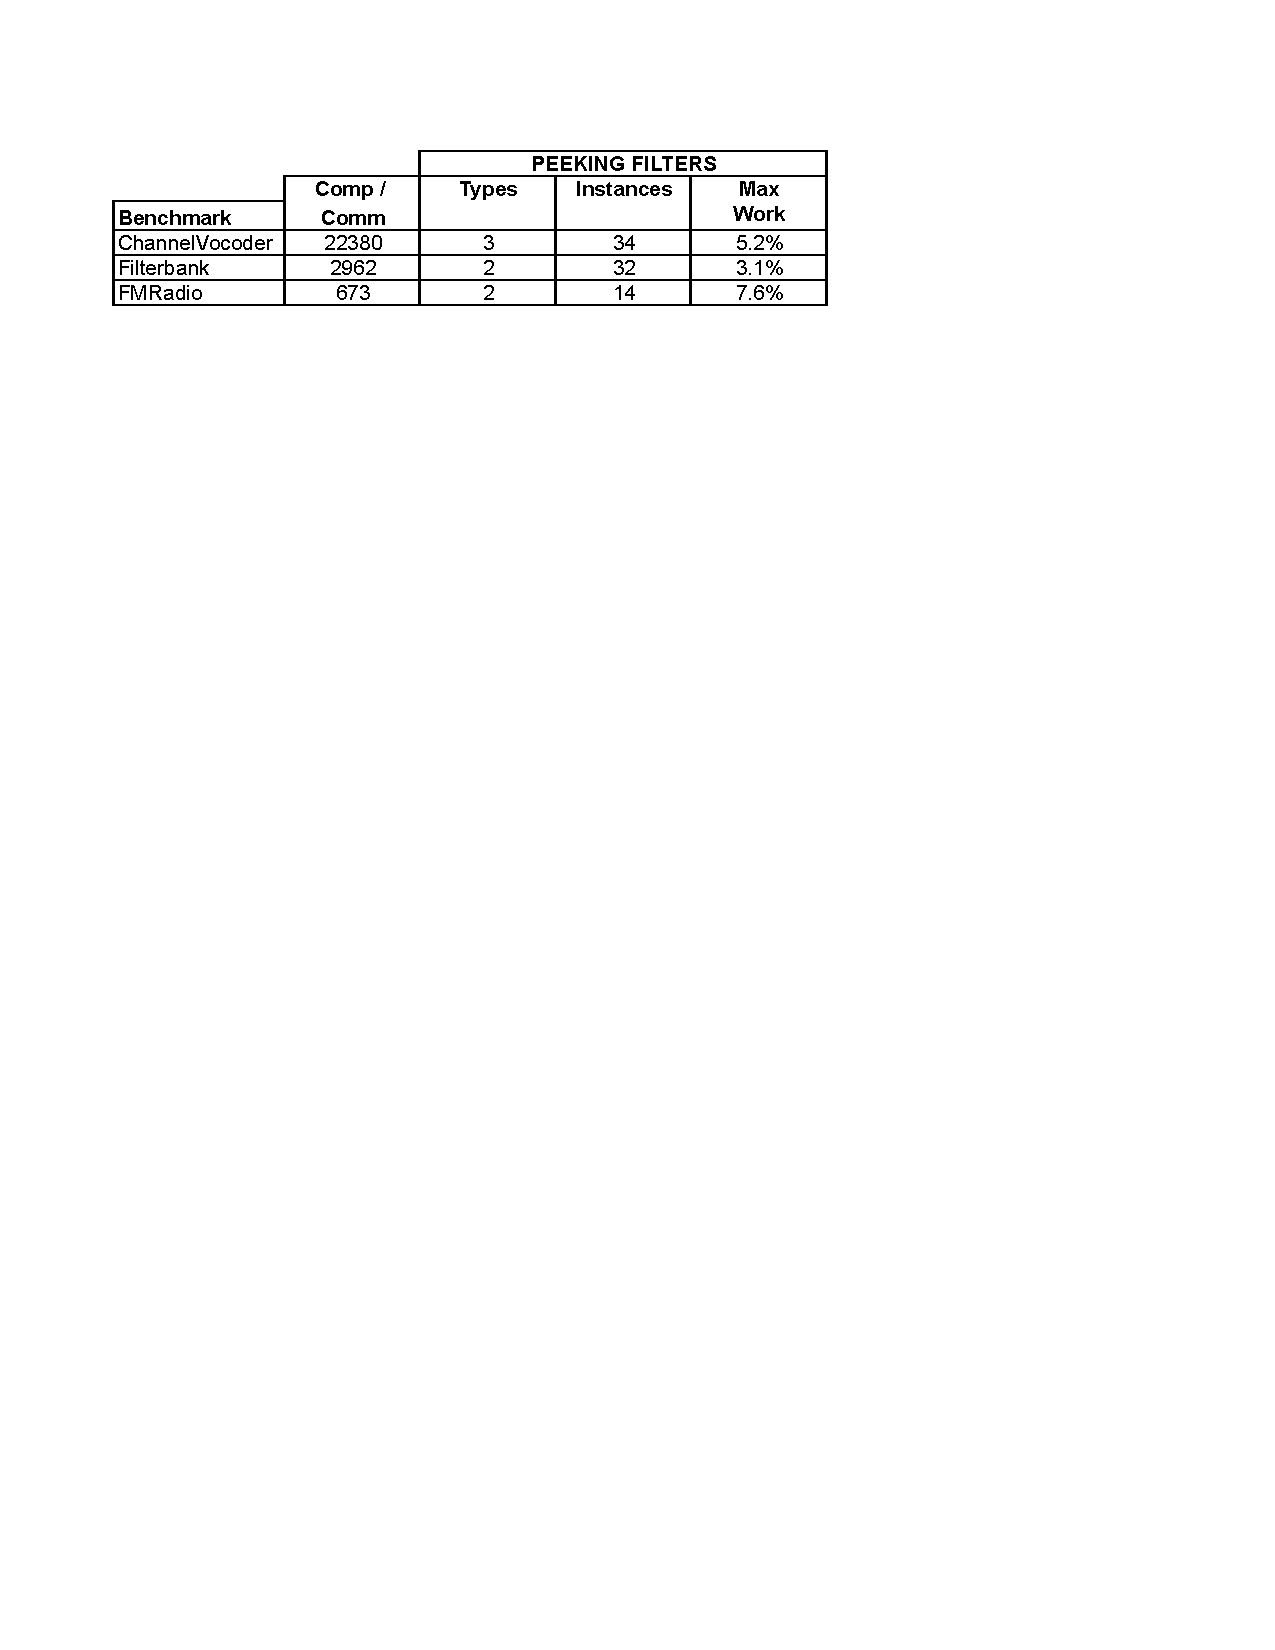
\includegraphics[width=3.3in]{figures/bench-char.pdf}}

\noindent ``Comp/Comm'' provides a static estimation of the
amount of computation to communication ratio by statically estimating the total
work of all the filters and dividing by the number items communicated
for the programmer-conceived graph's steady-state.  The remaining
statistics give the number of peeking filters types, number of peeking
filters instantiated at runtime, and a static estimation of the maximum
work in the single most loaded peeking filter.

We target 2 multicore architecture with different communication
mechanisms.  The Tilera Corporation's TILE64 Processor is a 64 core
system on a chip~\cite{tilera}.  Each core is an identical three-wide
VLIW. The code generated by the StreamIt
compiler for the TILE64 processor follows the remote store programming
(RSP) model~\cite{rsp10} in which each process has a private address
space, but each process can award remote processes write access to
their local memory. When a producer process has write access to a
consumer process's memory, the producer communicates directly with the
consumer via store instructions whose destination is an address in the
consumer's shared memory.  Communication is initiated by the producer,
and is fine-grained.  The consumer reads directly from it's local
memory (L2) when accessing input.

Our symmetric multiprocessor target is a 16-core architecture that is
comprised of four Intel Xeon E7350 multicore processors.  Each processor
is a 64-bit, quad-core with two dual-core dies.  Each die contains a 4
MB L2 cache shared across the two cores.  The front-side bus is clocked
at 1066 MHz.  We utilize the cache coherency mechanism of the
architecture for communication between cores. 

Through empirical experimentation on FMRadio, Filterbank, and
ChannelVocoder, we have settled on $T_{\mt{sharing}} =.10$ and
$T_{\mt{apply}} = 0.05$. These constants are the sweet stop for the two
architectures employed in the experimentation, being a good compromise
between buffer size and inter-core communication.

% \begin{figure*}[t]
% \centering
% \subfigure[]{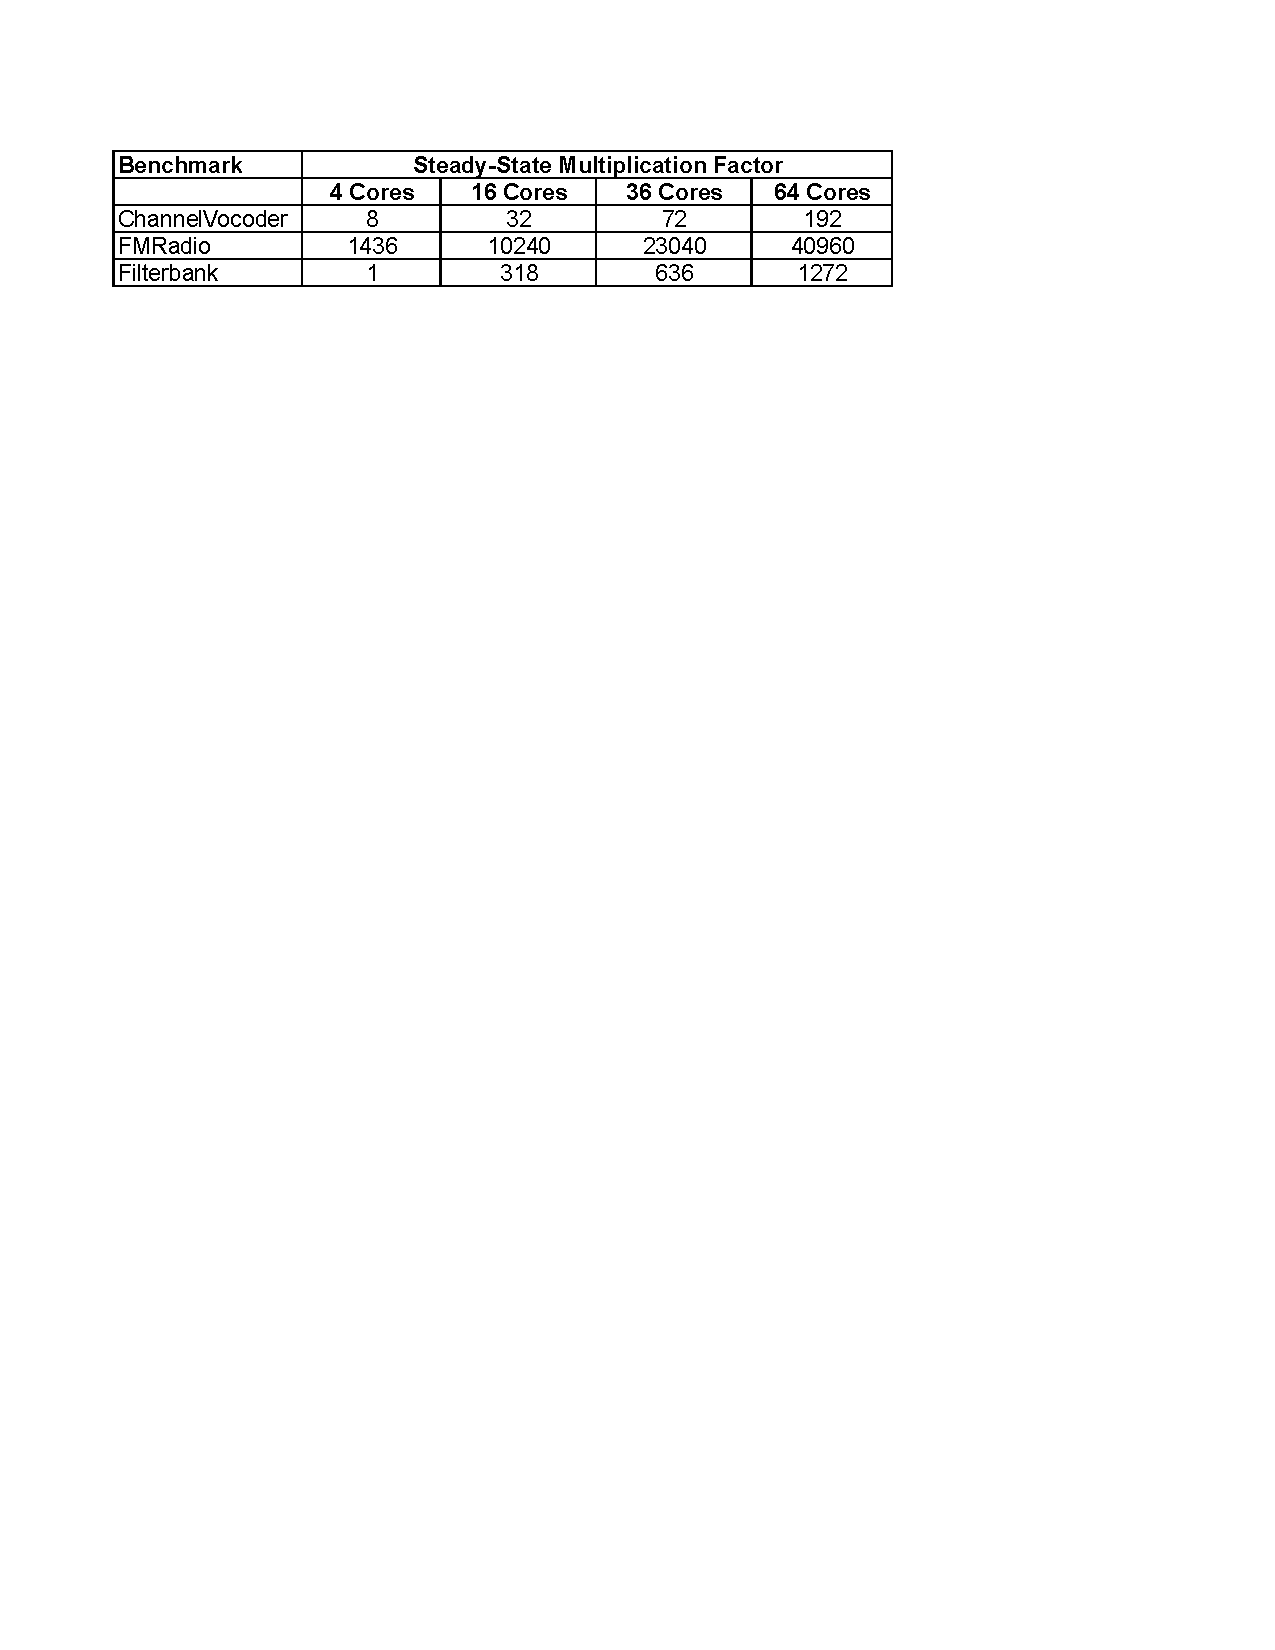
\includegraphics[width=3.7in]{figures/mult-table.pdf}} \\
% \subfigure[]{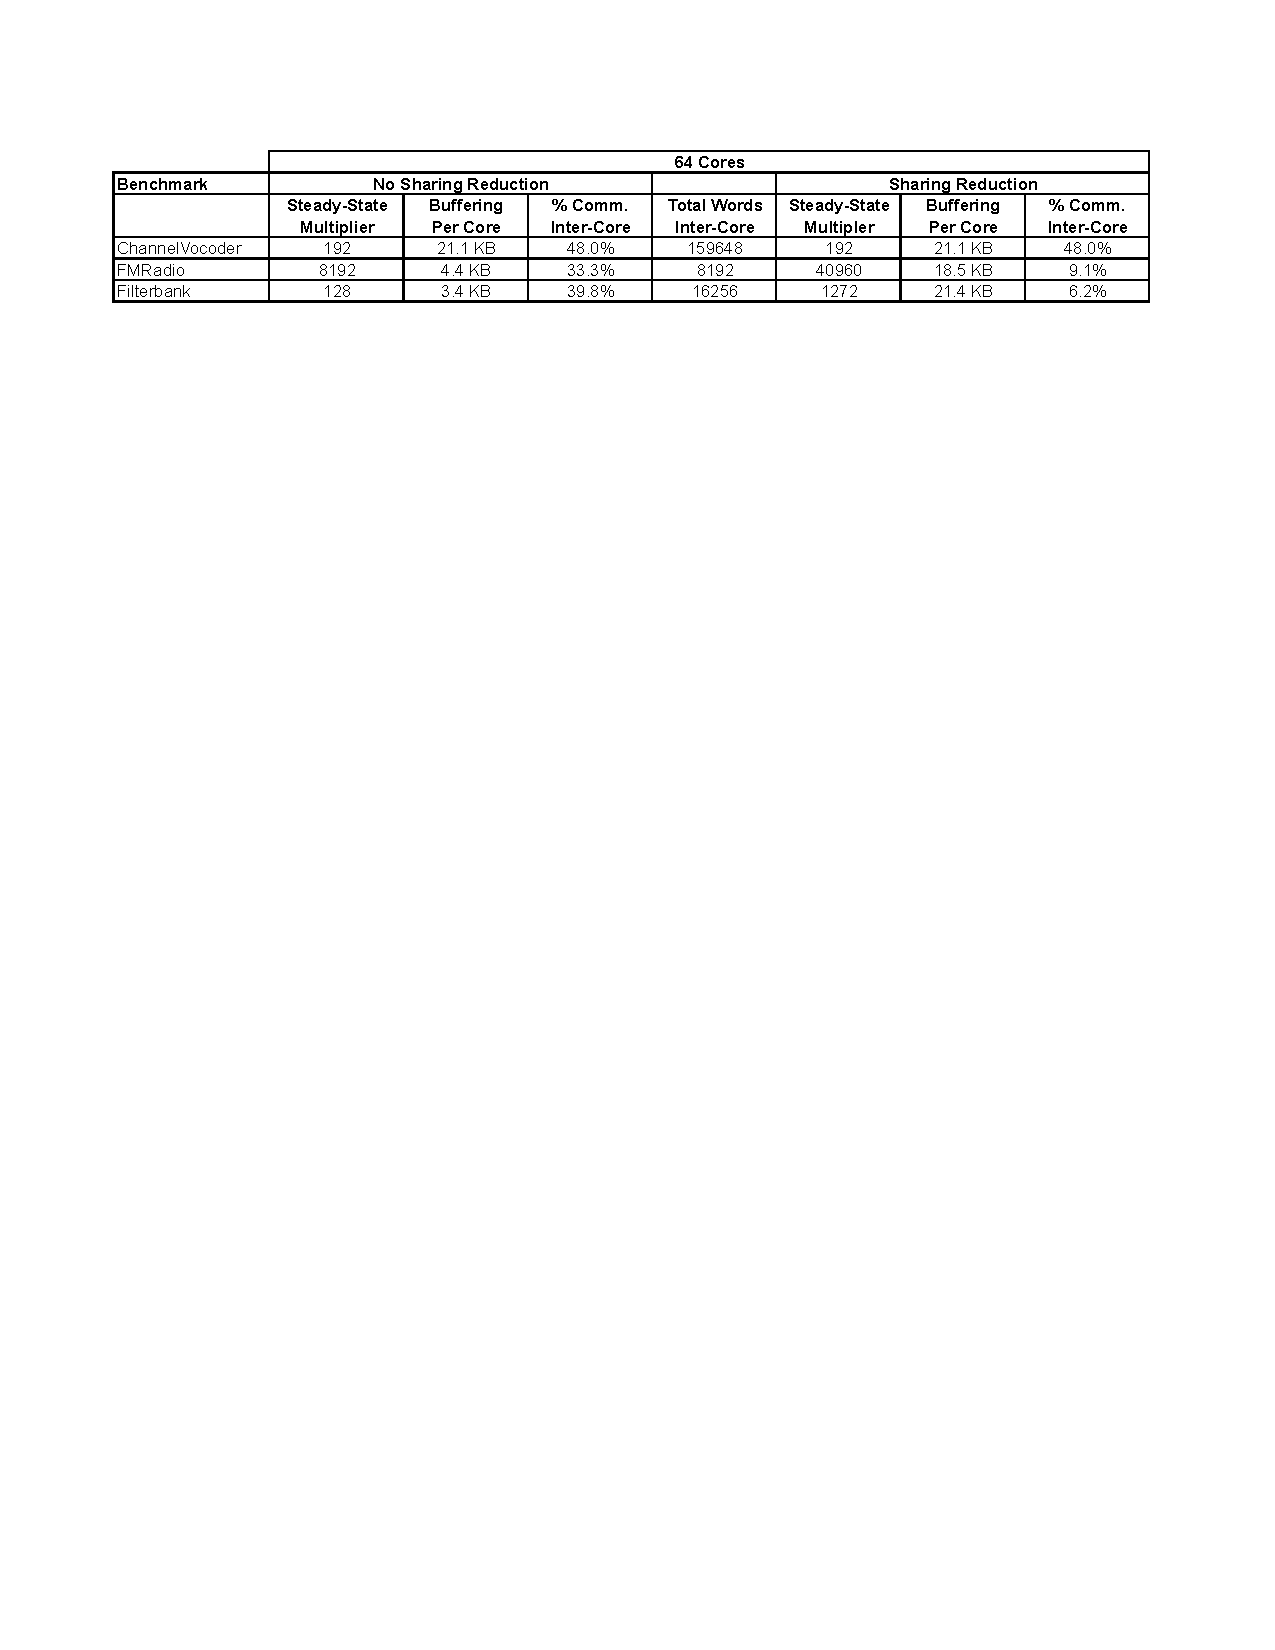
\includegraphics[width=6in]{figures/64-core-table.pdf}}
% \caption[Communication, multiplier and buffering statistics for
% benchmarks.]{
% Communication, multiplier and buffering characteristics for
% benchmarks: (a) gives the steady-state multipliers calculated for
% sharing reduction, (b) compares the steady-state with and without
% sharing reduction. 
% \label{fig:fission-table}}
% \end{figure*}

\begin{figure*}[t]
\centering
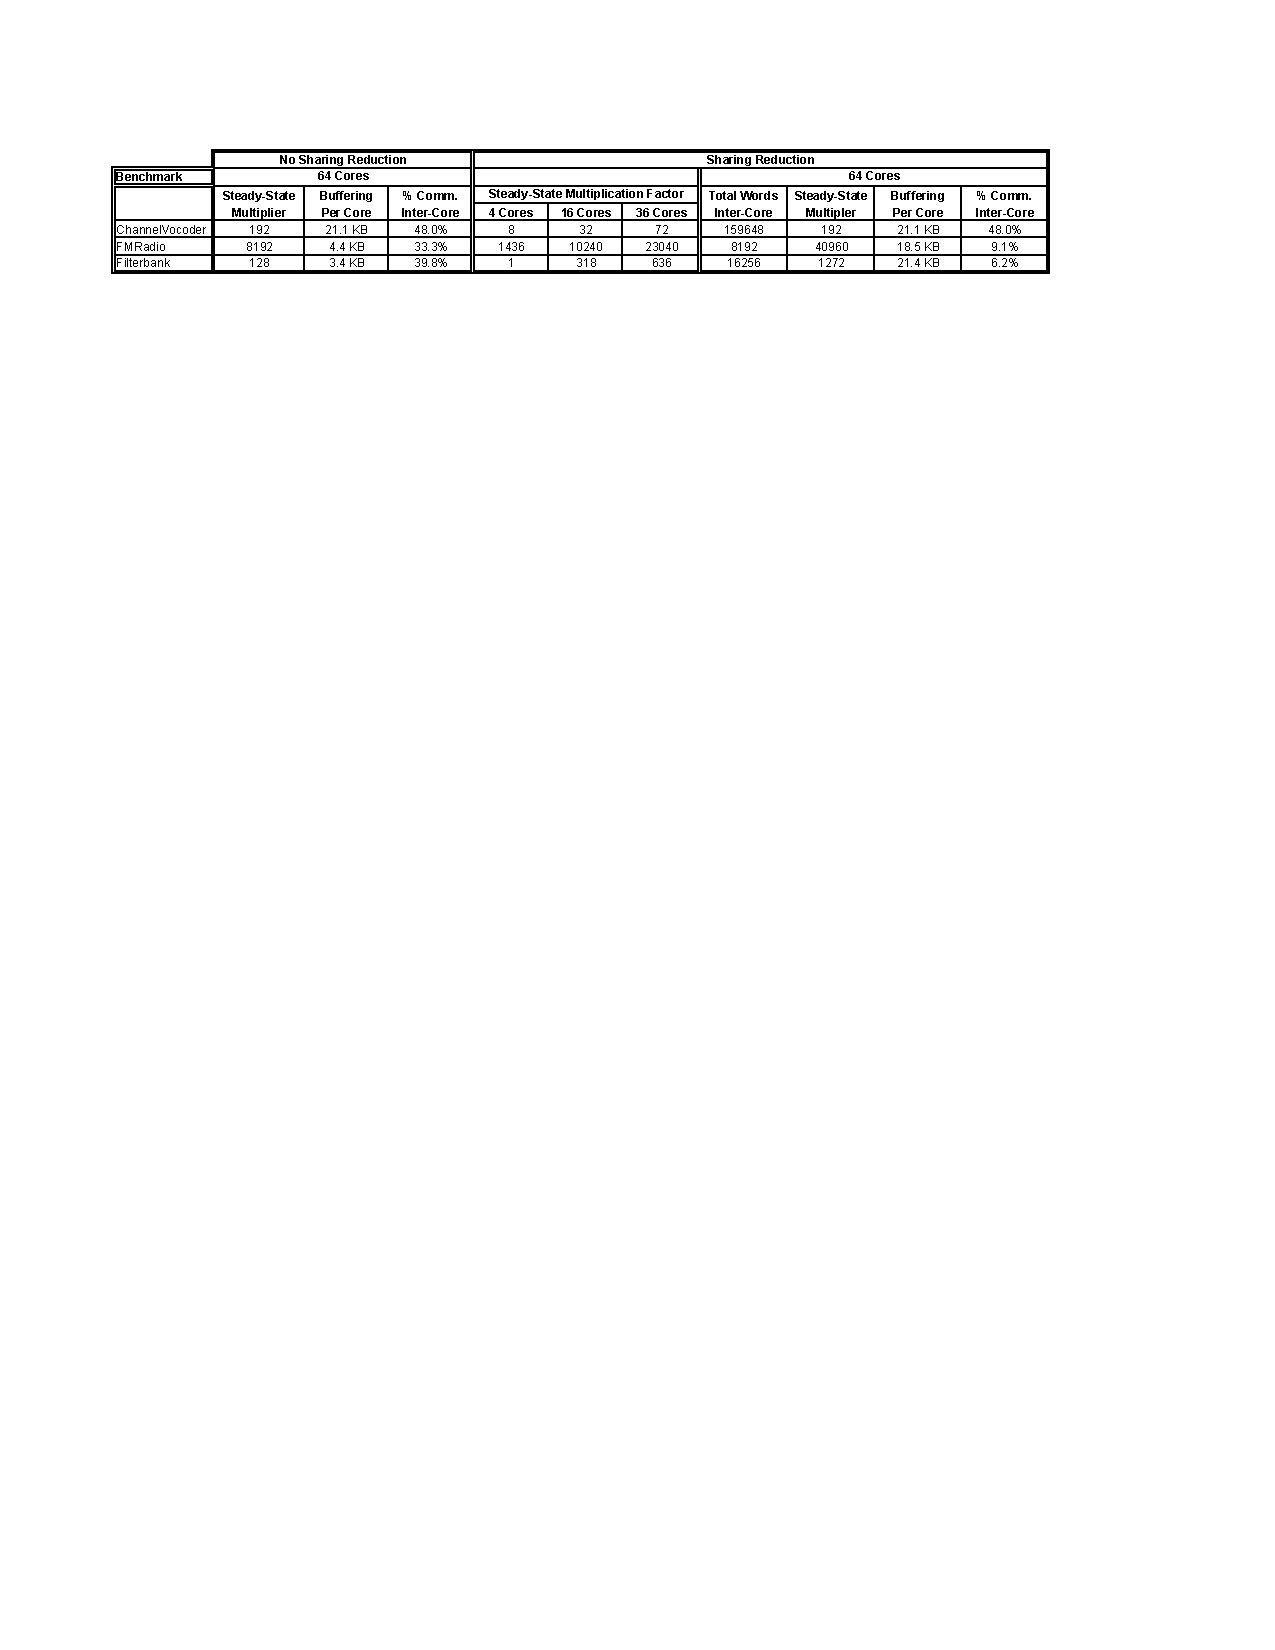
\includegraphics[width=6.1in]{figures/big-table.pdf}
\caption{\label{fig:big-table}  Steady-state multiplicity, buffering,
  and communication for fission with and without sharing reduction.}
\end{figure*}

% \begin{figure}[t]
% \centering
% 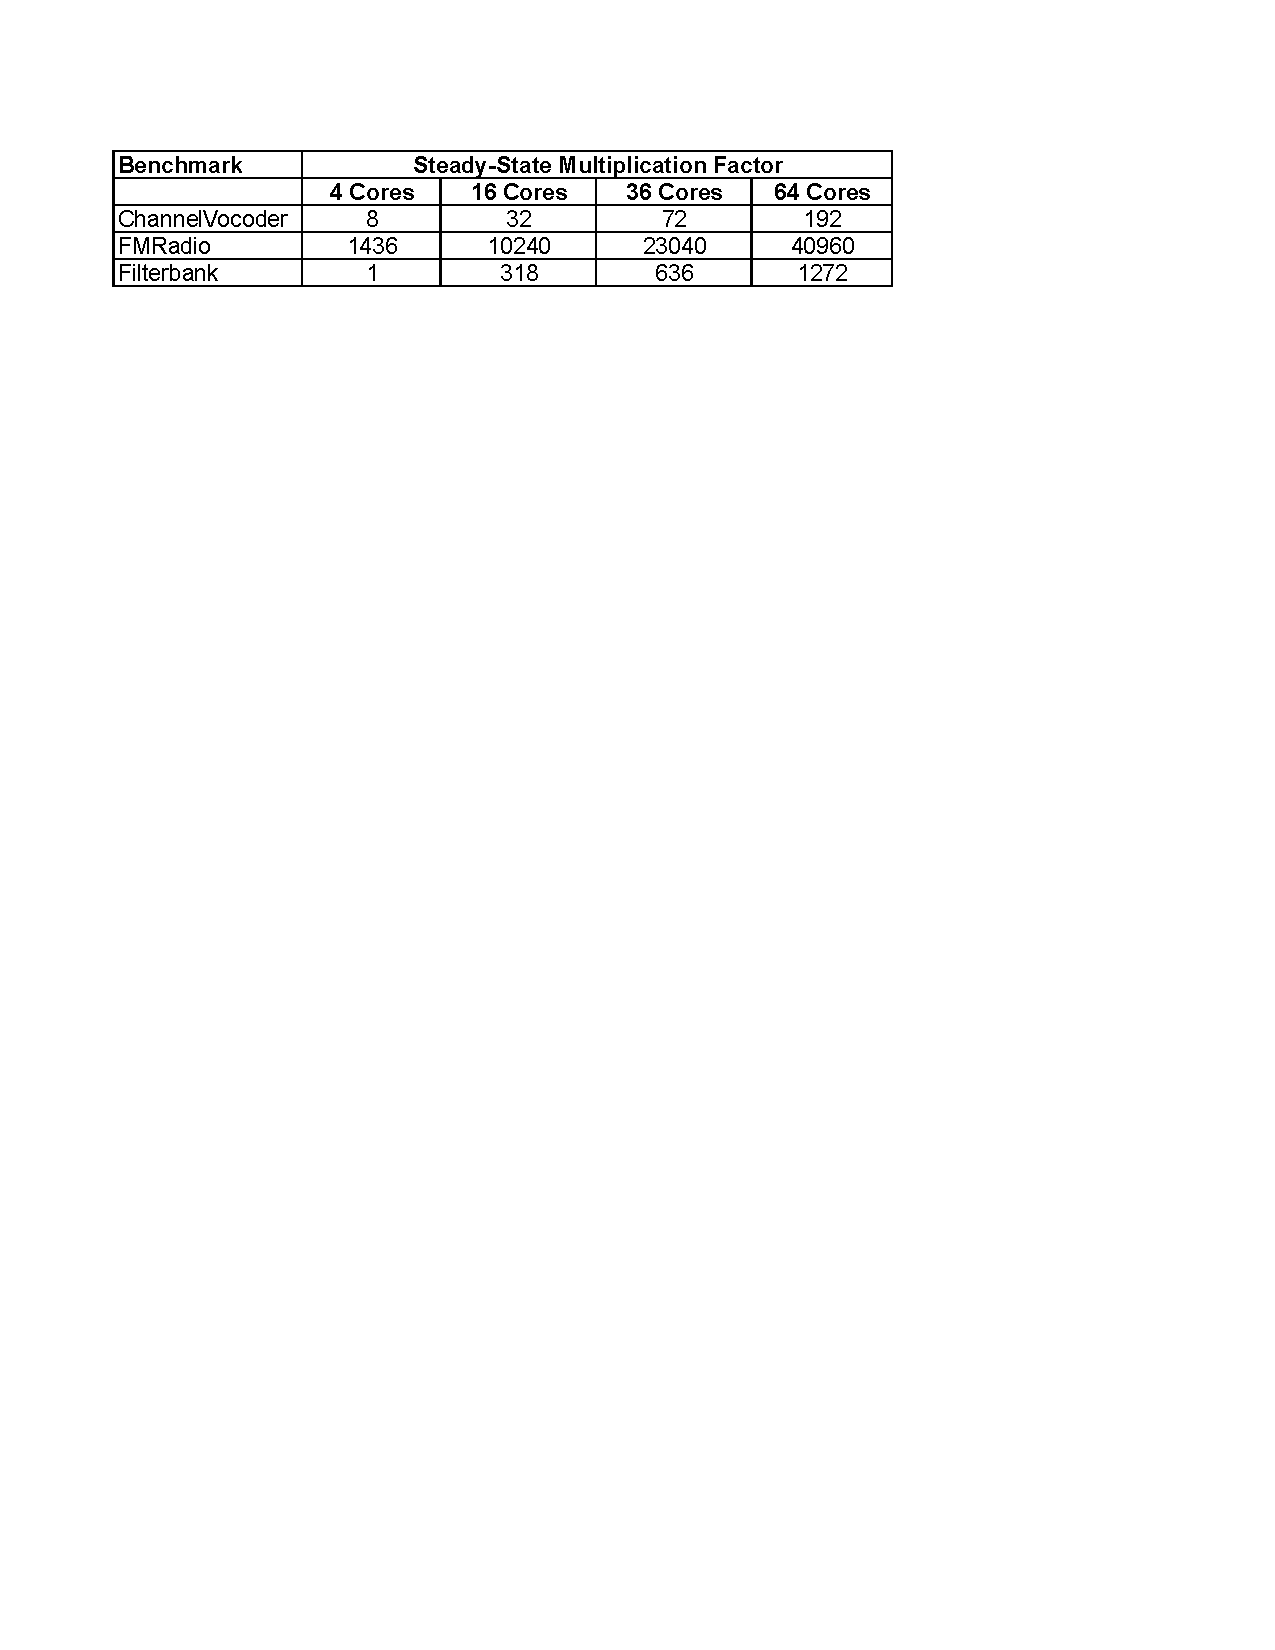
\includegraphics[width=3.3in]{figures/mult-table.pdf}
% \caption{\label{fig:mult-table}  The steady-state multipliers calculated for
% sharing reduction.}
% \end{figure}

% \begin{figure*}[t]
% \centering
% 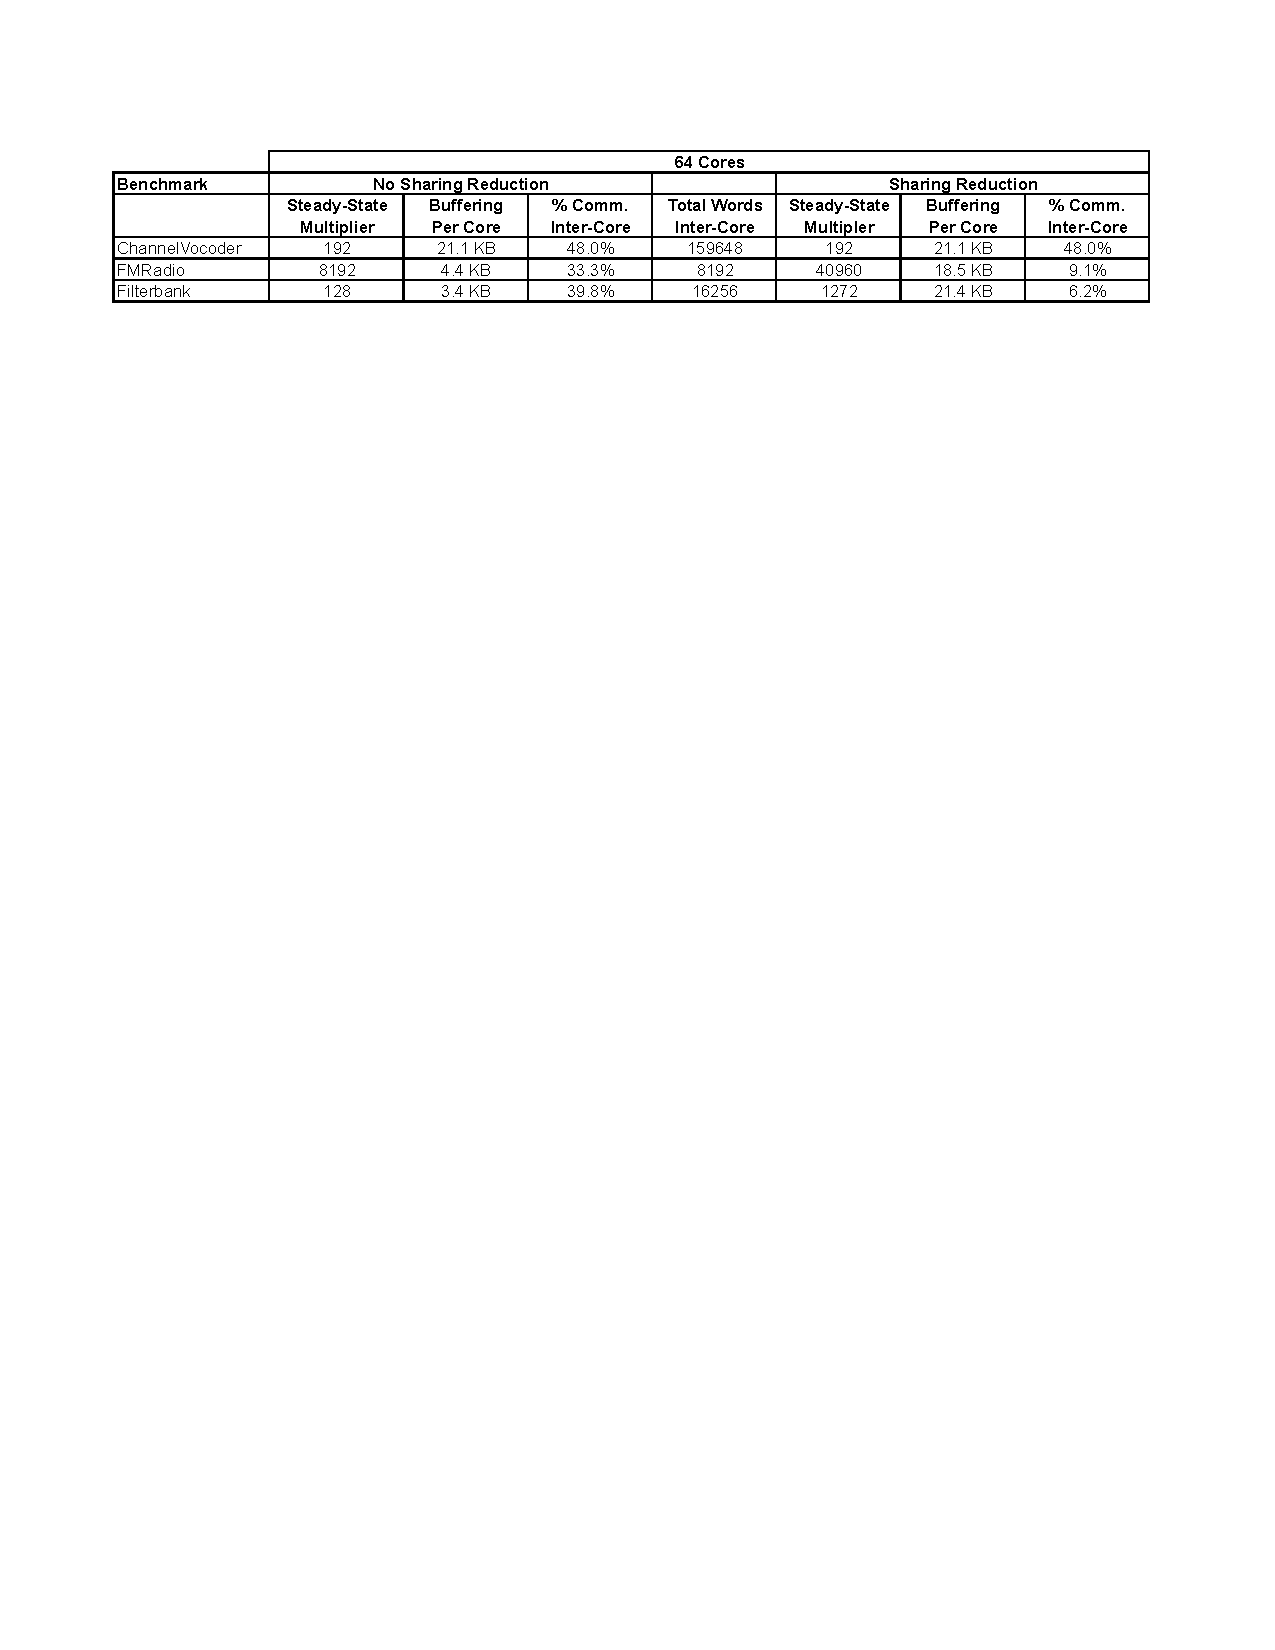
\includegraphics[width=6in]{figures/64-core-table.pdf}
% \caption{ Multiplier, buffering and communication for the steady-state with and without
% sharing reduction. 
% \label{fig:fission-table}}
% \end{figure*}

Figure~\ref{fig:big-table} compares the steady-state with and
without sharing reduction for a 64-core mapping, as well as gives the
constant $c$ calculated by sharing reduction for 4, 16, and 36.  The
factor is larger for FMRadio because one filter has $C(f) \gg o(S,
f)$.  The multiplication factor affects both latency and buffer sizes
adversely.  The application designer will have to decide if the
latency of these techniques can be borne given the application
criteria.  The total buffering requirement is increased when the
steady-state is increased.  However, since we are then fissing, the
buffer is divided amongst the fission products, and the {\it per-core}
buffering requirement is unaffected by the increase.  For example,
FMRadio, has a per-core 18 KB buffering requirement across all
configurations (4, 16, 36, and 64 cores).  This requirement fits in
the per-core L2 size of 64 KB for the Tile64.

 For ChannelVocoder,
sharing reduction has no effect because most of the peeking filters do
not satisfy $T_{\mt{apply}} = 0.05$ because of differing fission
factors between producers and consumers.  For the peeking filters that do,
the steady-state multiplier required for legal general fission for the
graph is enough to assure $T_{\mt{sharing}}$ is met.  Even though
sharing reduction has no effect for ChannelVocoder, general fission
avoids the 38\% of total items that were unnecessary duplicated by
DupDec.

For FMRadio and Filterbank, sharing reduction leads to significant
decreases in the percentage of total items communicated inter-core for
each steady-state.  The buffer requirement is increased an average of
5.2x for these benchmarks.  The total number of words communicated
inter-core during each steady-state is the same, with and without
sharing reduction.  However, the steady-state is greater in the
sharing reduction case, thus producing more outputs.

\begin{figure}[t]
\centering
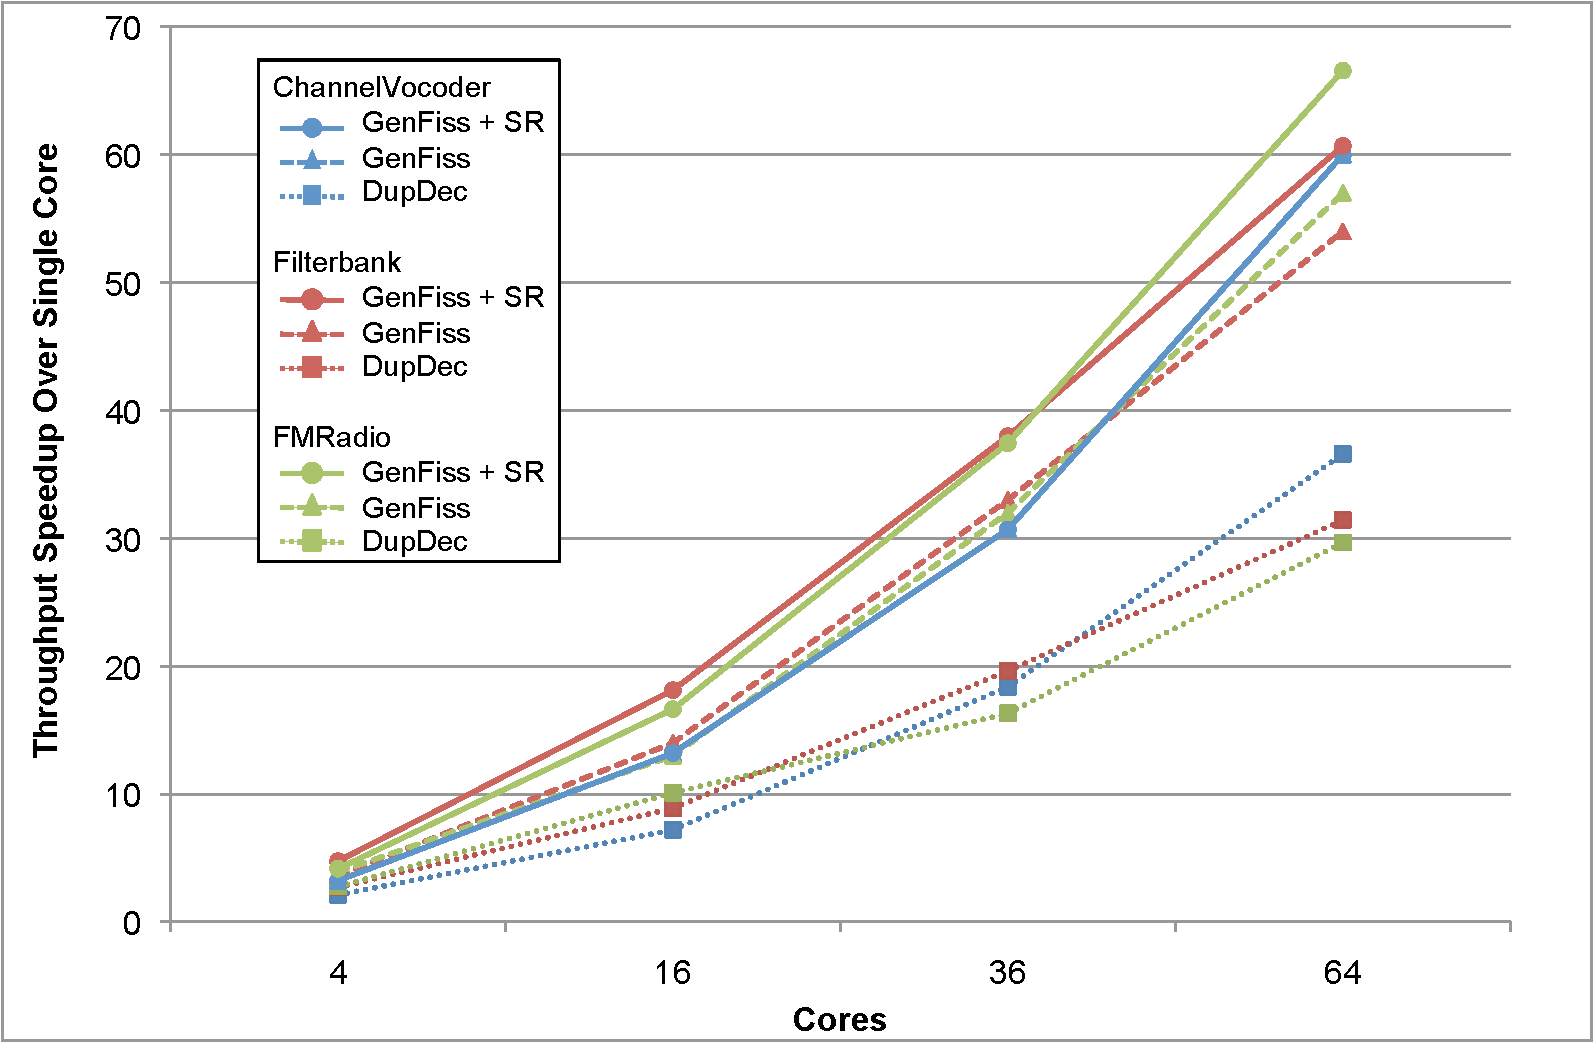
\includegraphics[width=3.3in]{figures/tilera-chart.pdf}
\caption[Comparing the fission techniques on the TILE64.]{
  Evaluation for DupDec versus general fission versus general fission with sharing reduction
  4, 16, 36, and 64 cores on the TILE64.  \label{fig:tilera-chart}}
\end{figure}

Figure~\ref{fig:tilera-chart} gives the performance results for the
Tilera TILE64 architecture.  We present results for DupDec, general
fission, and general fission with sharing reduction for 4, 16, 36, and
64 core configurations, with throughput normalized to single-core
throughput.  General fission with sharing reduction outperforms
DupDec by an average of 1.8x for the three benchmarks when targeting
64 cores. The average 64-core speedup over single core is 62.3x for the
general fission plus sharing reduction for these three benchmarks.

FMRadio experiences the most significant gain from general fission
plus sharing reduction over DupDec (67x versus 30x, respectively, for
64 cores).  FMRadio has the lowest computation to communication ratio
of the 3 benchmarks.  Furthermore, each filter of is fissed by the
number of cores targeted.  For 64 cores, each filter is fissed 64
ways.  DupDec must perform a global all-to-all communication involving
all 64 cores between each level of the graph!
 
ChannelVocoder achieves a 60x speedup for general fission over a
single core.  This is not perfectly linear because of the parallel
mapping; asymmetries exist between the extent of task parallelism and
the number of cores (see~\ref{mgordon-asplos06}).  The speedup over
DupDec (1.62x) is more modest because the width of many of the
fission applications is 3, so DupDec is duplicating input data to
groups of 3 filters.  Filterbank is similar, the width of fission is 4
for all filters when targeting 64 cores.

Sharing reduction is required to achieve scalable speedups for both
FMRadio and Filterbank.  For FMRadio, sharing reductions leads to a
17\% speedup increase for 64 cores.  This because sharing reduction
significantly reduces the number of remote write store instructions
required per output.  This affects FMRadio because of its low
computation to communication ratio.  Sharing reduction sees a 12\%
increase on Filterbank, as Filterbank has a larger computation to
communication ratio.

\begin{figure}[t]
\centering
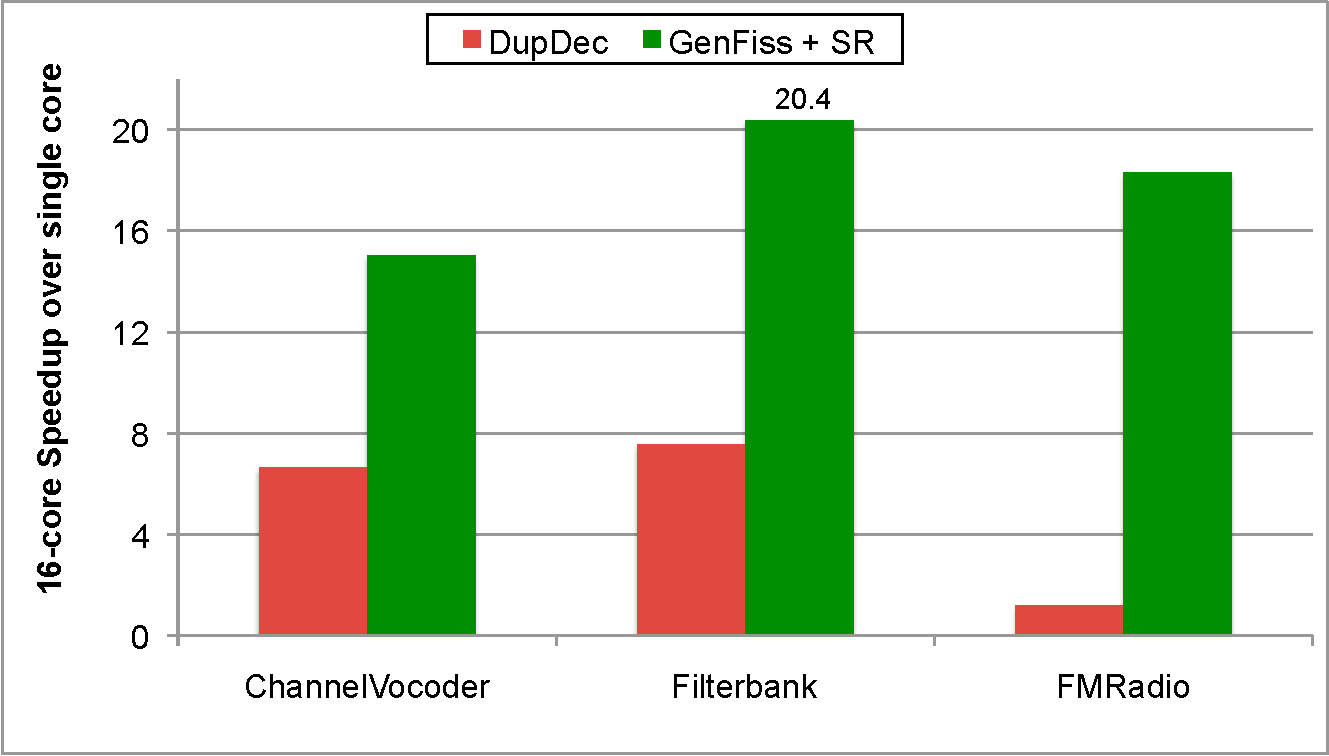
\includegraphics[width=3.3in]{figures/smp-chart.pdf}
\caption[Comparing the fission techniques on the 16-core SMP.]{
  Evaluation for DupDec versus general fission with sharing reduction
  for the 16-core SMP architecture.  \label{fig:smp-chart}}
\end{figure}

Our techniques enable scalable parallelization, with a mean speedup of
17x for our 3 benchmarks on the SMP.  Figure~\ref{fig:smp-chart} gives
the 16-core speedup comparison for DupDec versus general fission with
sharing reduction for our target SMP architecture.  The mean speedup
increase for general fission with sharing reduction over DupDec is
6.7x.  FMRadio again sees the largest speedup increase in the
comparison at 13.0x.  The reasons for this large speedup are similar
as given in the previous section.  However, the SMP communication
mechanism is not as efficient as the TILE64, thus general fission with
sharing reduction gives a greater speedup because reducing inter-core
communication has more impact.

  \section{Related Work}
\label{sec:related}

% BILL

%Signal~\cite{Signal}, 
%Lucid~\cite{Lucid77}, and
%Occam~\cite{Occam}, and Sisal \cite{sisal}.
%Parallel Haskell~\cite{ph}
In addition to StreamIt, there are a number of stream-oriented
languages drawing from domains such as functional, dataflow, CSP and
synchronous programming~\cite{survey97}.  The Brook language is
architecture-independent and focusses on data
parallelism~\cite{brook04}.  Stream kernels are required to be
stateless, though there is special support for reducing streams to a
single value.  Stream\-C/Ker\-nel\-C is lower level than Brook;
kernels written in KernelC are stiched together in StreamC and mapped
to the data-parallel Imagine processor~\cite{imagine03ieee}.  SPUR
adopts a similar decomposition between ``microcode'' stream kernels
and skeleton programs to expose data parallelism~\cite{spur05samos}.
Cg exploits pipeline parallelism and data parallelism, though the
programmer must write algorithms to exactly match the two pipeline
stages of a graphics processor~\cite{cg03}.  Compared to these
languages, StreamIt places more emphasis on exposing task and pipeline
parallelism (all the languages expose data parallelim).
%and on sliding window operations (filters that peek).  
By adopting the synchronous dataflow model of execution~\cite{lee87},
StreamIt focusses on well-structured programs that can be aggressively
optimized.  The implicit infinite loop around programs is also a key
StreamIt characteristic that enables the transformations in this
paper.  Spidle is also a recent stream language that was influenced by
StreamIt~\cite{spidle03}.
%and Lucid Synchrone~\cite{Lucid-Synchrone}.
%Synchronous languages which
%target embedded applications include Esterel~\cite{Esterel},
%Lustre~\cite{Lustre}, and Additional

Liao et al. map Brook to multicore processors by leveraging the affine
partitioning model~\cite{liao06brook}.  While affine partitioning is a
powerful model for parameterized loop-based programs, in StreamIt we
simplify the problem by fully resolving the program structure at
compile time.  This allows us to schedule a single steady state using
flexible, non-affine techniques (e.g., simulated annealing) and to
repeat the found schedule for an indefinite period at runtime.
Gummaraju and Rosenblum map stream programs to a general-purpose
hyperthreaded processor~\cite{gummaraju05micro}.  Such techniques
could be integrated with our spatial partitioning to optimize per-core
performance.  Gu et al. expose data and pipeline parallelism in a
Java-like language and use a compiler analysis to efficiently extract
coarse-grained filter boundaries~\cite{du03sc}.  Ottoni et al. also
extract decoupled threads from sequential code, using hardware-based
software pipelining to distribute the resulting threads across
cores~\cite{ottoni05decoupled}.  By embedding pipeline-parallel
filters in the programming model, we focus on the mapping step.

%%%%%%%%%%%%%%%%%%%%%%%%%%%%%%%%%%%%%%%%%%%%%%%%%%%%%%%%%%%%%%%%%%%%%

Previous work in scheduling computation graphs to parallel targets has
focused on partitioning and scheduling techniques that exploit task
and pipeline parallelism~\cite{SDFSched, SDFSched2,may87communicating,
DAGSched, pipeline-sdf}.  Application of loop-conscious
transformations to coarse-grained dataflow graphs has been
investigated.  Unrolling (or ``unfolding'' in this domain) is employed
for synchronous dataflow (SDF) graphs to reduce the initiation
interval but they do not evaluate mappings to actual
architectures~\cite{unfolding,unfolding2}. Software pipelining
techniques have been applied to SDF graphs onto various embedded and
DSP targets~\cite{bakshi99,chatha-02}, but has required programmer
knowledge of both the application and the architecture. To our
knowledge, none of these systems automatically exploit the combination
of task, data, and pipeline parallelism.  Furthermore, these systems
do not provide a robust end-to-end path for application
parallelization from a high-level, portable programming language.

%% Previous work on instruction-level software pipelining has focused
%% mostly on scheduling machine instructions in a loop via modulo
%% scheduling~\cite{rau81,lam-softpipe}.  The algorithms devised must
%% account for tight resource constraints and complex instruction
%% dependences. Our software-pipelining problem is much less constrained,
%% enabling us to employ a simple greedy heuristic.  

%% Furthermore, a traditional modulo scheduling algorithm is not needed
%% because we have an implicit loop barrier at the end of each
%% steady-state.  ILP compilers for clustered VLIW
%% architectures~\cite{Bulldog,Multiflow,lee98spacetime,qian02} must
%% partition instructions and assign them to clusters as part of the
%% instruction scheduling. Clustering is analogous to our application of
%% filter fusion in our software pipelining algorithm.

  \section{Conclusion}
\label{sec:conclusion}

In this paper, we describe the StreamIt compiler for the Raw
architecture.  The stream graph of a StreamIt program exposes the data
communication pattern to the compiler while the lack of global
synchronization frees the compiler to radically reoganize the program
for efficient execution on the underline architecture. The StreamIt
compiler demonstrates the power of this flexibility by totally
reoganizing large programs for better load balance. We were able to
map many of programs on to the Raw processor and obtain good
performance.

We introduce a collection of optimizations, vertical and horizontal
filter fusion, vertical and horizontal filter fission and filter
reordering transformations, that can be used to restructure stream
graphs.  We show that by applying these transformations we can map a
high-level stream program, written to reflect the composition of the
application, onto Raw and achieve good processor utilization and load
balance, leading to a factor of three speedup on two applications.

Unlike all previous streaming languages, the structured streams of
StreamIt makes it possible for us to approach the optimization and
parallelization problems in a very systermatic manner. It enables us
to define multiple optimizations -- targetting different constructs
and requirements -- and to compose them them in a hirearchical manner.

The ability to do global transformations across multiple filters, that
may have originated from very different parts of the application,
makes it possible for the compiler to find optimization opportunities
that may ellude even an experience programmer.  Such capabilities
enables the programmers to write protable streaming applications and
map them efficiently onto any given architecture. This has the
potential of creating a programming standard for emerging
communication exposed architectures.  The StreamIt compiler takes a
fist step towards this goal.


  
  \begin{small}
    \begin{singlespace}
      \bibliographystyle{abbrv}
      \bibliography{references}
    \end{singlespace}
  \end{small}
  
\end{document}
